\documentclass[a4paper]{scl-article}
\usepackage{amsmath,amssymb,graphicx, float}
\usepackage{listings}
\usepackage{xcolor}

% Render the Philippine peso glyph (U+20B1) safely under pdflatex.
% On engines that natively support Unicode (XeLaTeX, LuaLaTeX) this
% declaration is benign; pdflatex would otherwise reject the codepoint.
\DeclareUnicodeCharacter{20B1}{Php\,}

\lstdefinestyle{terminal}{
  basicstyle=\ttfamily\footnotesize,
  backgroundcolor=\color{gray!8},
  frame=single,
  framerule=0.4pt,
  rulecolor=\color{gray!40},
  framesep=4pt,
  xleftmargin=8pt,
  xrightmargin=8pt,
  breaklines=true,
  columns=fullflexible,
  keepspaces=true,
  showstringspaces=false,
  captionpos=b,
  aboveskip=10pt,
  belowskip=10pt
}
\lstset{style=terminal}

\begin{document}

\title{Dynamic Authorization in Digital Payments: A (t, n) Threshold Signature Protocol for Securing QR Code Transactions}


\author{Denzell Dy, Nathaniel Feliciano, Gerard Salao \\ 
Susan Pancho-Festin, Juan Felipe Coronel \\ 
Computer Security Laboratory - Department of Computer Science \\ College of Engineering, University of the Philippines Diliman \\ Quezon City 1101, Philippines}




\maketitle
\section{Review of Related Literature}
\label{header:rrl}
\subsection{Introduction to QR Codes}
\label{sect:rrl_1}
\paragraph{}Due to their convenience, mobile payment systems have become ubiquitous to the point where political economists have claimed that the end of the cash era is only a matter of time \cite{rulyfayrizqi2019}. Among the mobile payment systems that have emerged globally, Quick Response (QR) codes are considered the leading system, accounting for 85\% of all mobile payments \cite{tu2022}. Nevertheless, the price of QR exploitation has correspondingly risen, especially since the COVID-19 pandemic surge \cite{sonowal2024}. This consequently calls for a more secure implementation of said system, which can be attained through a thorough investigation of its history, constituents, and existing implementations.


\subsubsection{Definition and History of QR Codes}
\label{sect:rrl_1a}
\paragraph{}Developed in 1994 by Masahiro Hara and his team at DENSO WAVE, a Toyota subsidiary \cite{densoQR}, QR codes are a type of matrix code consisting of a two-dimensional barcode with black squares arranged in a square grid on a white background \cite{worldbank2021}.  It is primarily the improved version of one-dimensional barcodes. Standard one-dimensional barcodes pose a concerning security risk since they can be easily interpreted by the human eye due to their single-directional nature. They also raise an inconvenience with scanner readings as they can only be read at specific angles. Apart from these, barcodes are storage-inefficient as they can only hold up to 20 numerical digits. In sum, these concerns make barcodes inefficient in terms of security, space, and time. Fortunately, these three concerns were mitigated by Masahiro Hara’s development of the QR code. QR codes can hold up to 7,089 numeric characters, 4,296 alphanumeric characters, and 1,817 kanji characters of information \cite{sankara2012}. Due to the larger amount of data QR codes can hold, space efficiency is mitigated. This consequently reinforces security, as the increasing number of possible combinations exponentially increases complexity. Nevertheless, despite the increase in characters and combinations, QR codes still capture and decode nearly instantaneously, often less than 93 milliseconds at varying angles \cite{corpuz2025}. 

\subsubsection{Structure, Versions, and Error Correction in QR Codes}
\label{sect:rrl_1b}
\paragraph{}QR codes are generally structured into seven (7) specific parts as shown in~\ref{fig:qr-structure}.  The big squares around the three (3) corners of the QR code are called $^1$position markers, which help identify the code’s orientation. The $^2$alignment marker aids in correcting distortion, allowing QR codes to be scannable at any angle. $^3$Timing patterns assist in helping scanners understand the size of the code’s embedded data. $^4$Format info holds information about error tolerance and mask pattern. The $^5$quiet zone helps a scanner locate position markers. The $^6$version number tells the user about the version of a scanned QR code, as different versions mean different capabilities, mainly in terms of capacity. Lastly, the rest of the squares or $^7$modules, covering the remaining area of the QR code, consist of the actual embedded data \cite{uniqode2025}. Version-wise, there are 40 different versions of QR codes with varying data capacities. Version 1 consists of 21 $\times$ 21 modules, from which 133 of these modules can be used for storing the actual encoded data. On the other hand, Version 40, which produces the largest QR code, consists of 177 $\times$ 177 modules, allowing a ceiling of 23,648 actual encoded data and hence, 7,089 numeric characters, 4,296 alphanumeric characters, and 1,817 kanji characters of information \cite{worldbank2021, steemanQR}. 

\paragraph{}Hitherto, the most commonly used version of a QR code is Version 2 \cite{krombholz2014}. Behaviorally, QR codes have two (2) variations: static and dynamic. Static QR codes, as their name suggests, have their data fixed, whereas the only way to change the encoded information is to generate an entirely new QR code. Contrarily, dynamic QR codes’ data can be changed or updated after the code is generated \cite{tekale2024, worldbank2021ch5}. This means that the QR code itself does not contain the data. It merely serves as a reference to an online location where the data is stored. Furthermore, error correction in QR codes is achieved through its basis on Reed-Solomon Code \cite{bajaj2024, reed1960}. These very codes are responsible for allowing data from QR codes to be decoded even if the codes become partially covered or damaged. In this mechanism, there are four standardized correction levels, namely L (Low 7\%), M (Medium 15\%), Q (Quartile 25\%), and H (High 30\%). Each correction level approximates the percentage of code words that can be restored [9]. For example, error correction level L can tolerate up to 7\% unreadable modules. Likewise, higher error correction levels enhance reliability but reduce the amount of usable data storage as extra modules are used for the said levels. More so, accessing the encoded data is done via a smartphone’s built-in camera, which decodes it using the phone’s internal QR code reader software \cite{krombholz2014}. To stabilize this decoding process, masking is also employed, which ensures an equal distribution between the black and white modules of the code. The appropriate mask is simultaneously chosen by the encoding software of the device upon the code’s creation \cite{pasala2024}.

\begin{figure}[h!]
  \centering
  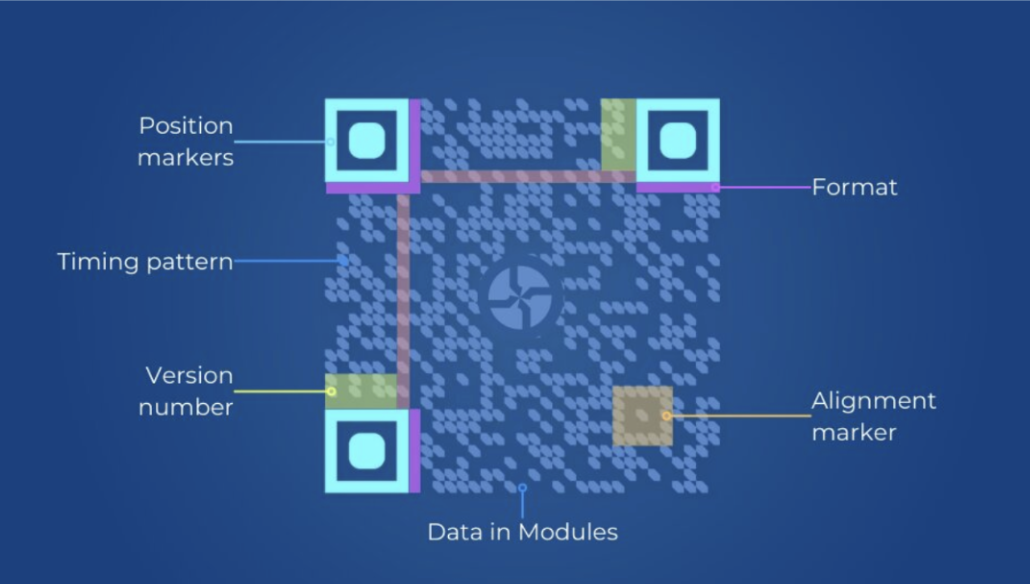
\includegraphics[width=0.6\textwidth]{images/qr-structure.png}
  \caption{QR code general structure \cite{uniqode2025}}
  \label{fig:qr-structure} % this is the "name" of the figure
\end{figure}

\subsubsection{QR Code Applications}
\label{sect:rrl_1c}
\paragraph{}As QR codes have essentially doubled the primary capacities of barcodes, such as reading speed, accuracy, security, and overall functionality, it has taken the world by storm \cite{tu2022}. In fact, because of its global presence, it has gained specific data types based on the various types of information it is set to hold. Accordingly, smartphone QR code reader software mentioned earlier in \ref{sect:rrl_1b} has also been adjusted by manufacturers to adapt to this reality of varying QR code data types. These data types are categorized by contact information, calendar events, e-mail addresses, phone numbers, geo locations, Short Message Service (SMS), texts, WiFi networks, URLs, and much more \cite{worldbank2021}. In addition to that, backed by China’s application of QR codes as a principal payment system, which is deemed to be beneficial to both customers and merchants, the payment system landscape has gradually skewed to QR code transactions \cite{worldbank2021ch5}. This, in turn, has made QR codes the chief initial mechanism for push and pull payments, e-commerce transactions, bill payments, credit/debit card dependencies, authentication dependencies, and even the basis of service requests for conglomerate businesses \cite{worldbank2021ch3}.

\subsection{QR Code Security Risks}
\label{sect:rrl_2}
\paragraph{}The very characteristics that have fueled the global integration of QR codes: their high data capacity, ease of generation, and role as a primary payment gateway, simultaneously present a vast surface for cyber-exploitation. Because the underlying architecture discussed in Section \ref{sect:rrl_1} prioritizes convenience and speed, they often lack inherent authentication. Consequently, to propose robust security enhancements, it is necessary to first categorize and analyze the specific risks and attack vectors that have emerged alongside their widespread adoption.

\subsubsection{Quishing (QR Phishing) and Cloning}
\label{sect:rrl_2a}
\paragraph{}Attackers may clone authentic QR codes, often using stickers to paste over existing benign codes in public areas like billboards \cite{averin2020}. These malicious codes redirect users to legitimate-looking phishing sites designed to steal sensitive personal information, credentials, corporate logins, or financial data. This practice is sometimes specifically referred to as "quishing" when the malicious QR code is distributed via email \cite{canada2024}. Attackers can also modify specific modules of an existing QR code (e.g., changing white modules to black using a pen) to alter the encoded content without replacing the entire code. This behavior is shown in~\ref{fig:quishing-img}, where changing just a few of the white and black modules redirected and overwrote the original QR code's URL to a malicious one \cite{yong2019}. 

\begin{figure}[h!]
  \centering
  
\includegraphics[width=0.6\textwidth]{images/quishing.png}
  \caption{Quishing showcase \cite{yong2019}}
  \label{fig:quishing-img} % this is the "name" of the figure
\end{figure}

\subsubsection{Malware Payloads}
\label{sect:rrl_2b}
\paragraph{}In logistics and payment systems, unsanitized or compromised (i.e., hacked) encoded data (e.g., QR codes or barcodes) can be exploited to launch attacks against automated processes. Common threats include SQL injection, where malicious queries manipulate backend databases, and command injection, where encoded data is executed as unsafe parameters \cite{kieseberg2010}. More advanced techniques, such as XML External Entity (XXE), format string exploits, server-side include (SSI) injection, and local file inclusion or directory traversal (LFI/DT), can also be leveraged to access sensitive files or disrupt operations \cite{averin2020}.

\subsection{QR Code Risk Mitigation}
\label{sect:rrl_3}
\paragraph{}Given the diverse range of attack vectors—from physical manipulation like quishing to sophisticated digital exploits such as SQL injection, a multi-layered defense strategy is required. Research into countermeasures against these vulnerabilities focuses on strengthening the code's integrity through (or a combination of) cryptography, artificial intelligence, image processing, and user interface optimization.

\subsubsection{Cryptographic and Steganographic Approaches}
\label{sect:rrl_3a}
\paragraph{}Fundamentally, visual cryptography involves splitting the original QR code into an arbitrary number \textit{n} of distinctly shared images or “shadows” \cite{bhardwaj2024, naor1995}. It adopts the standard (\textit{k}, \textit{n}) aspect of cryptography, meaning that if fewer than \textit{k} distinct shadows are stacked and aligned correctly, the original QR code cannot be retrieved \cite{ibrahim2021}. Unlike conventional encryption that secures only the QR code’s payload, visual cryptography conceals the code’s visual structure itself, preventing unauthorized reconstruction.

\paragraph{}A visual cryptographic approach to enhancing QR code security involves embedding “shadows” within the original QR code, creating a new “stacked” QR code that combines both the original QR code and its shadows. These shadows are composed of a subdivision or transposition of the original QR code image, which essentially allows for the masking of the QR code under the shadows \cite{li2020}. The aforementioned approach can be used together with a “carrier” QR code, creating two QR codes, where data retrieval is accomplished through one QR code being stored in a cloud server, which will be used to retrieve the original QR code and subsequent data when the carrier QR code is scanned upon payment. Multiple schemes or methods can be used to achieve the approach mentioned above, such as the utilization of the XOR mechanism of Reed-Solomon (RS) codes, with additional concealment by pre-embedding the shadows in a background image, or using the error correction mechanism of the QR code as the embedding mechanism itself before running it through the XOR mechanism mentioned above \cite{lu2017}.

\paragraph{}This approach can also be augmented with steganography (hiding data within another object), which allows the embedding of the QR data to be hidden in the QR image itself. This is implemented through algorithms such as Least Significant Bit (LSB) and Random Data Hiding (RDH) \cite{bhardwaj2024}. Since the QR data will be completely hidden in the image generated, decryption and reconstruction must be performed on the image to get the data hidden from the approach \cite{ibrahim2021}. Moreover, steganography can also be combined with Linear Feedback Shift Register (LFSR) processing. Along with separating the RGB channels of the QR code image using the Rubik’s cube principle and encrypting them with AES, this multi-encryption scheme demonstrated a high security score of 99.94\% in resisting statistical attacks \cite{narayanan2024}.

\paragraph{}Traditional key-based encryption can also provide security to QR codes. The Secured QR Code (SQRC) is designed to safeguard personal and confidential information during scanning. SQRC encrypts sensitive data with a code key and integrates it directly into the QR code. Only specialized readers equipped with the matching secure key can decrypt its content, ensuring that unauthorized devices cannot access protected data \cite{saranya2016}. Another approach is through re-encryption, where data that was previously encrypted on the user end and embedded into the QR code is decrypted and re-encrypted through a proxy server, which is then decrypted again at the destination. This approach ensures that no security compromises that occur during the communication expose any secret data in the QR code \cite{akhil2016}.

\paragraph{}A related enhancement is digital watermarking. Compared to visual cryptography, watermarking prioritizes tamper detection and authenticity verification rather than data concealment. A proposed watermarking scheme with multi-level authentication involves dividing the QR code into a Region of Interest (ROI), the preserved intact, and a Region of Non-Interest (RONI) where security tags and backup data are embedded \cite{lei2021}.

\paragraph{}Across the reviewed studies in this subsection, a common trend emerges: visual cryptography is consistently leveraged as a foundation for creating secure QR codes, often in combination with steganographic techniques and multi-layer encryption. This indicates its perceived importance in QR code security frameworks. Apart from this, the metrics used to evaluate these approaches, such as mean squared error (MSE), peak signal-to-noise ratio (PSNR), structural similarity index measure (SSIM), and entropy score \cite{bhardwaj2024, narayanan2024, sofyan2024}, are relatively uniform across the literature in this section, suggesting that these benchmarks form the baseline standards for assessing QR code security solutions. Furthermore, recent watermarking-based schemes highlight the need for even more robust frameworks capable of withstanding extreme image degradation while preserving hidden authentication and recovery data \cite{lei2021}. 

\paragraph{}Future directions thus point toward exploring more metrics to evaluate the encryption and distortion-reduction techniques that ensure the QR image remains visually and statistically indistinguishable from its original form, or even supports greater data embedding capacity without sacrificing image quality or scannability. Such advancements will be crucial for ensuring QR codes remain secure and verifiable even under real-world distortions or malicious manipulation.


\subsubsection{Machine Learning and Deep Learning Algorithms}
\label{sect:rrl_3b}
\paragraph{}While cryptographic and steganographic approaches aim to mitigate attacks on QR codes by strengthening their structure, machine learning and deep learning approaches aim to identify and flag QRs that have been tampered with or are actually malicious in nature \cite{sahoo2017}.

\paragraph{}For these approaches, traditional and deep learning models such as ResNet, VGG, and conventional CNNs are used to distinguish or classify benign and malicious QR codes using computer vision. These models are then evaluated through different metrics, such as accuracy and F1-score, to find the model that best classifies (benign or malicious) the QR data given to them \cite{lourenco2023}. 

\paragraph{}While vision-based models are effective, many of the most predictive features come not from the QR image but from its content payload. Thus, natural language processing (NLP) techniques often offer stronger leverage, with features like URL length, suspicious keywords, and word patterns proving useful for detecting deceptive QR code links. Researchers developed QsecR, a secure Android scanner that uses rule-based URL analysis and external API checks to flag suspicious sites, achieving 93.50\% accuracy \cite{rafsanjani2023}. Another study, meanwhile, applied machine learning models such as Random Forest, Logistic Regression, and LSTM to lexical and behavioral URL features, finding that textual indicators strongly predict malicious \cite{tayachi2025}. Combining both rule-based and machine learning methods, the AP3X Secure QR Codes Infrastructure integrates multiple ML models (RF, LightGBM, XGBoost, NN) with external API analyses, reaching over 96\% detection success \cite{rivas2025}. 
 


\paragraph{}These classification models are usually used in real-time solutions, such as QR scanners, which makes it imperative that real-time performance and efficiency also be prioritized for easy accessibility and integration on different types of devices, ranging from different commercial and retail QR scanners to smartphones \cite{rafsanjani2023}.

\paragraph{}From the models mentioned above, it is documented that the random forest model approach for identifying malicious URLs was deemed to be the best in terms of efficiency, accuracy, generalizability, and real-world viability. Contrastingly, deep learning models, despite doing well in terms of efficiency and accuracy metrics \cite{lourenco2023}, fell short in real-time deployment due to computational complexity \cite{tayachi2025}. 

\paragraph{}As such, these classification models are normally implemented in real-time detection applications \cite{rafsanjani2023} and integrations to existing QR code scanners as a layer of security, which makes a balance between both efficiency and accuracy a metric to maximize. Future studies can implement adversarial training to counter evasion techniques and conduct real-time detection optimizations for mobile applications \cite{tayachi2025}. 


\subsubsection{Dynamic Security Methods}
\label{sect:rrl_3c}
\paragraph{}Unlike cryptographic and classification ways of mitigation, dynamic QR codes can also provide security in QR code systems. Compared to static QR codes that remain unchanged, dynamic QR codes are generated in real-time for each transaction and can include temporary or device-specific data \cite{choudhary2023}. In today’s mobile payment systems, users often make transactions by generating a dynamic QR code, which functions much like a barcode that merchants scan to complete payment \cite{garnaik2022, wei2024}. This dynamic nature not only improves transaction speed and flexibility but also adds a layer of protection against fraud, since a copied or replayed QR code quickly becomes invalid. 

\paragraph{}Building on the idea of dynamic protection, Garnaik and Ryoo \cite{garnaik2022} proposed a method that safeguards payment QR codes by rotating them at random angles. During a transaction, the code displayed on the user’s screen continuously changes orientation, and the payment is verified only if the scanner detects three consecutive rotations that match the values stored on the server. This approach prevents attackers from using screenshots or recorded videos, since a static image would fail to align with the required rotation pattern.

\paragraph{}Advancing this concept even further, Wei et al. \cite{wei2024} developed UniQR, which ties each QR code to the physical movement and orientation of the user’s device. When a user generates a payment QR code, their phone records its position and angle through built-in sensors and embeds this “pose” information within the code. The scanner then compares this embedded pose data with what it observes through the camera. If the two do not match, as would be the case with a stolen or screenshot QR code, the payment is rejected. 

\paragraph{}Overall, most studies have focused on using dynamic QR codes as a means of enhancing payment security. However, these approaches primarily emphasize the security of QR code usage rather than the security of QR code generation itself. Since the generation process can still be vulnerable to hacking or tampering, integrating cryptographic algorithms, as discussed in \ref{sect:rrl_3a}, during QR code creation presents a promising direction for future research and experimentation.

\subsubsection{Synthesis: A hybrid cryptographic solution to address identified gaps}
\label{sect:rrl_3d}
\paragraph{}The preceding review has shown that work on QR‑code security clusters into three complementary strands: (1) image‑level protections such as visual cryptography and watermarking that conceal or tag QR data; (2) content‑level defenses and detection via machine learning that flag malicious or tampered codes; and (3) operational measures achieved through dynamic QR generation that limit replayability in payment flows. Each strand provides valuable mitigations, yet none, in isolation, fully addresses the joint requirements of robust authenticity, resistance to key compromise, and practical deployability in joint‑account payment settings.

\paragraph{}Visual cryptography and steganographic schemes effectively hide or split QR imagery, but their reliance on image stacking and carrier channels introduces operational complexity and does not by itself remove the fundamental single‑key failure mode of many current payment systems. Similarly, ML‑based scanners excel at detecting tampered or malicious payloads, yet they are reactive (detection after tampering) and do not provide cryptographic proof that a scanned code was authorized by the legitimate account holders. Dynamic QR methods improve freshness and replay resistance, but implementations that rely on a single signing key or on device‑specific pose/orientation checks remain vulnerable if that key or device is compromised. Collectively, these observations point to a persistent gap highlighted in the literature: the need for a provably secure, multi‑party authorization mechanism that (a) preserves practical convenience for payments, (b) prevents single‑point compromise, and (c) integrates naturally with dynamic QR workflows.

\paragraph{}To bridge this gap, we propose a hybrid approach that synthesizes threshold cryptography with dynamic QR generation and lightweight proxy‑mediated coordination. The approach is motivated by four central insights from the reviewed works:


\begin{enumerate}
    \item \textbf{Distribute trust, eliminate single-point failure.} Shamir’s secret sharing and subsequent threshold signature literature demonstrate that a signing capability can be split among $n$ parties so that any authorized subset of size $t$ suffices to produce a valid signature, while coalitions smaller than $t$ cannot forge it \cite{shamir1979, desmedt1988, gennaro2007}. Applying $(t,n)$ threshold signatures to payment authorization removes the single-key vulnerability inherent in many dynamic QR systems.
    
    \item \textbf{Compact, aggregatable proofs for QR payloads.} Pairing-based signature schemes such as BLS provide compact signatures and support non-interactive aggregation of partial signatures into a single verifiable signature (thus keeping QR payload size and scanning latency low) \cite{boneh2001}. Aggregation is therefore a practical choice for embedding authorization proofs into dynamic QR codes.
    
    \item \textbf{Operational coordination without key exposure.} Prior work on proxy-assisted re-encryption and secure relays indicates that a lightweight proxy can coordinate message distribution and session keys while never learning secret key material, enabling efficient multi-party signing in real networks \cite{chen2011, ruffing2014}. The proxy model preserves end-to-end cryptographic assurances while simplifying real-time coordination across participant devices.
    
    \item \textbf{Freshness and multilevel authentication.} Nonce and timestamp mechanisms are simple, well-studied tools to prevent replay, and can be combined with a policy engine that maps transaction risk (e.g., monetary amount) to required threshold $t$, thereby implementing multilevel authentication in a principled manner (higher risk calls for larger $t$). This synthesizes watermarking/ROI ideas for authentication with dynamic QR freshness guarantees described in the dynamic security literature.
\end{enumerate}

\paragraph{} 
On this basis, the present study adopts a $(t, n)$ Threshold Signature Scheme (TSS) implemented using an aggregatable signing primitive (e.g., BLS), together with nonce/timestamp freshness, and a proxy relay for encrypted coordination. In the resulting design, each transaction message 
\[
M = \{\textit{Merchant\_ID}, \textit{Amount}, \textit{Timestamp}, \textit{Nonce}\}
\] 
is signed via distributed partial signatures $i$ (computed locally by key-share holders) and combined into a single final signature $F_{\text{sig}}$ that the verifier can efficiently validate against the joint public key. 

\paragraph{}This hybrid construction directly addresses the three main deficiencies identified in Section \ref{sect:rrl_3}: it 
\begin{enumerate}
    \item replaces single-key dependency with threshold assurance;
    \item embeds compact, verifiable authorization into the dynamic QR payload (mitigating reliance on post-hoc ML detection); and
    \item retains operational practicality via proxy-assisted coordination and simple replay controls.
\end{enumerate}

The methodology and formal protocol that implement this synthesis are further described in Chapter \ref{header:methodology}.

\section{Methodology}
\label{header:methodology}
\subsection{Study Conception}
\label{sect:meth1}
\paragraph{}Since dynamic QR codes are obviously superior to static QR codes due to their improved transaction speed and flexibility, as well as an added layer of protection against fraud since replayed QR codes quickly become invalid, this study will focus on strengthening them further. The study aims to do these by addressing the implicit gaps mentioned in the study’s RRL:

\begin{enumerate}
    \item Leveraging the threshold nature of visual cryptography, but applying it to digital signature shares instead of visual shares.

    \item Strengthening proxy-server-based approaches such as SQRC, including:
    \begin{enumerate}
        \item Increasing the number of key shares to reduce single points of failure.
        \item Retaining the proxy server to coordinate secure message relay.
    \end{enumerate}

    \item In the same nature as (1) and (2), watermarking and multilevel authentication will be incorporated through the use of:
    \begin{itemize}
        \item nonce
        \item timestamp
        \item multiple key shares
    \end{itemize}
\end{enumerate}


\subsection{System Architecture}
\label{sect:meth2}
\paragraph{}
The proposed system utilizes a hybrid cryptographic and dynamic QR-based authorization framework that integrates threshold cryptography with secure proxy-mediated coordination. In line with gaps found in our related literature, its primary purpose is to provide decentralized, multi-party verification for digital transactions while mitigating replay and single-point-of-failure vulnerabilities found in static QR schemes (e.g., SQRC).

\paragraph{}
Its foundation lies in the (\textit{t}, \textit{n}) Threshold Signature Scheme (TSS) proposed by Shamir~\cite{shamir1979}, which successively expanded into distributed key signing protocols by Desmedt~\cite{desmedt1988} and Genarro~\cite{gennaro2007}. Briefly, the protocol divides the private signing key into \textit{n} distinct key shares, each stored securely within the personal device of an account member. From this, a transaction can only be validated when at least \textit{t} of these members jointly approve, preventing unilateral authorization or key compromise.

\subsubsection{System Entities}
\label{sect:meth2_a}
\paragraph{a.) Joint account (\textit{n}-members).}This entity represents a collaborative financial entity composed of \textit{n} authorized members. Each member possesses one (1) unique private key share ($k_i$), generated during account creation through a Distributed Key Generation (DKG) protocol. These key shares are never combined nor exposed, preserving forward secrecy~\cite{ruffing2014}.

\paragraph{b.) Payer (Coordinator).}  
This entity serves as the account member initiating the transaction request. The payer’s client module formulates the transaction message, determines the required signature threshold via an internal policy engine, and coordinates the distributed signing procedure.

\paragraph{c.) Proxy Server.}  
This entity serves as the secure, stateless intermediary that relays encrypted messages and partial signatures between the payer and participating co-signers. It facilitates synchronization and communication, but never accesses or stores any private cryptographic material. In essence, its primary function is to handle encrypted routing and quorum coordination efficiently while maintaining decentralized authorization integrity~\cite{chen2011}.

\paragraph{d.) Bank/Verifier.}  
The institutional endpoint that validates the aggregated signature. It checks message integrity, verifies the threshold-signed authorization, and ensures that replayed transactions (identified by duplicated nonces) are rejected.

\subsubsection{Cryptographic Components}
\label{sect:meth2_b}

\paragraph{a.) Distributed Key Generation (DKG).} 
Upon creating the joint account, the full private key, individual key shares ($k_i$) (by DKG), and the joint public key (\textit{PK}) are generated. Each threshold $t \le n$ defines a distinct key-sharing configuration, resulting in a unique set of keys corresponding to that threshold.

\paragraph{}The full private key serves as the basis for the privacy key shares, but never gets reconstructed due to forward secrecy from DKG. Due to this and the fact that there are multiple key shares, there would be no single point of failure (SPOF) to compromise the joint account. Moreover, the joint public key (PK) is likewise derived as a function of all private key shares and the elliptic curve generator \textit{g}, which will be further expounded in this section of the paper. In essence, DKG guarantees decentralization as it resolves SQRC’s SPOF while promoting forward secrecy since the full private key is impossible to reconstruct based on the distributed key shares.

\paragraph{b.) Public Key (\textit{PK}).}
This serves as the aggregate public key that represents the joint account’s cryptographic identity. Simply, it serves as the identity reference for the account, which checks the integrity of the shares and transaction message. To technically expound, it is mathematically defined by the summation given by:
\[
PK = \sum_{i=1}^{n} (\lambda_i \cdot k_i \cdot g)
\]

\noindent where:
\begin{align*}
k_i &= \text{member’s private key share}, \\
\lambda_i &= \text{Lagrange coefficient used in interpolation (depends on the set threshold } t), \\
           &\quad = \prod_{j \in S,\, j \neq i} \frac{0 - j}{i - j}, \\
g &= \text{generator point of the elliptic curve.}
\end{align*}

\paragraph{}To enlighten more on what \textit{g} is, it is the “origin” point from which all other points on the elliptic curve are derived. Multiplying the origin point \textit{g} by a scalar such as $k_i$ deterministically moves the point along the curve. Even so, this process of multiplication is computationally impossible to reverse, thereby enforcing forward secrecy, as cryptography must do.

\paragraph{c.) Transaction Message (\textit{M}).}
Each transaction is represented as a structured message:
\[
\textit{M} = \{\textit{Merchant\_ID}, \textit{Amount}, \textit{Timestamp}, \textit{Nonce}\}
\]

By using a \textit{Nonce}, transaction messages are ensured uniqueness, which prevents replay attacks. Additionally, adding a \textit{Timestamp} aids in temporal validity, as dynamic QR codes must definitely expire \cite{boneh2001}.

\paragraph{}Further, \textit{M} gets processed by the SHA-256 algorithm, which acts as the hash function for this study. \textit{M} then becomes a 256-bit hash value, which is its message digest, and is illustrated as follows:

\[
H(\textit{M}) = \text{SHA-256}(\textit{M})
\]

\paragraph{}This message digest, not the message itself, would later get signed, forming the signatures to be used in the methods.

\paragraph{d.) Policy Engine.}
This mechanism determines the required signing threshold \textit{t} based on the set \textit{Amount} found in the message \textit{M}. It essentially adjusts depending on the threshold set by the user. If transaction amounts escalate, risks increase. When risks rise, a higher threshold \textit{t} is ideated. To concisely visualize this at a high level, we can set $t=1$ for small payments, $t\ge2$ for high-value transfers.

\paragraph{e.) Threshold Signature Scheme (BLS).}
Each member with a key share that approves a transaction request computes a partial signature in the elliptic curve group using the equation given by:

\[
\sigma_i = H(\textit{M})^{k_i} = k_i \cdot H(\textit{M})
\]

It is important to note here that $H(M)^{k_i}$ denotes scalar multiplication of the hashed message point $H(M)$ by the private share $k_i$ in the elliptic curve group.

\paragraph{}If at least \textit{t} partial signatures are approved and collected, the Payer aggregates them using Lagrange interpolation:

\[
F_{\text{sig}} = \sum_{i=1}^{t} (\lambda_i \cdot \sigma_i)
              = \sum_{i=1}^{t} (\lambda_i \cdot k_i \cdot H(M))
\]

\paragraph{}This consequently produces a final signature ($F_{\text{sig}}$), which is equivalent to signing with the full private key. Note, however, that the final signature differs completely from the full private key, which means that no single key is ever reconstructed. This, again, showcases forward secrecy.

\paragraph{f.) Bilinear Pairing ($e(\cdot,\cdot)$).}

This is a mapping that serves as the basis for QR verification and validation, which concludes the study’s envisaged technology method. It is given by
\[
e: G_1 \times G_2 \rightarrow G_T
\]
between elliptic curve groups, which satisfies the bilinearity property \cite{john2023}:

\[
e(aP, bQ) = e(P, Q)^{ab}
\]

\noindent where:
\begin{align*}
P, Q & = \text{points on the elliptic curve}, \\
a, b & = \text{scalars (i.e., private keys $k_i$)}.
\end{align*}

This property of bilinear pairing ensures that the multiplication of points in the elliptic curve domain corresponds exactly to exponentiation in the target group $G_T$. To preface its core usage in the protocol flow to be discussed later, it would be used for final signature verification as such:

\[
e(F_{\text{sig}}, g) = e(H(M), PK)
\]

If both sides of the equation are equal, then the signature is valid and thus the transaction is permitted.

\paragraph{g.) Symmetric Encryption (AES-256-GCM).}
This encryption algorithm is the Advanced Encryption Standard (AES) algorithm with a 256-bit key and Galois/Counter Mode (GCM). Due to the nature of the message digest discussed earlier, a 256-bit key is consistent with the said algorithm \cite{abdalrahman2021}. Moreover, by using such, partial member signature sent over the proxy server will be attained, providing integrity and confidentiality as needed.

\paragraph{h.) Ephemeral Key Exchange (Diffie-Hellman).}
This establishes session keys for secure message passing, ensuring forward secrecy even if a future key becomes compromised. Likewise, it supports the dynamic QR code nature, whereas each generated key (private and public) expires when a new QR code gets generated. No two (2) live QR codes can use the same keys.




\subsection{Protocol Flow}
\label{sect:meth3}
\paragraph{}The proposed protocol consists of five (5) major cryptographic phases, coordinated via the proxy server. The corresponding diagram is depicted in Figure \ref{fig:method_diag}. % care %

\begin{figure}[H]
  \centering
  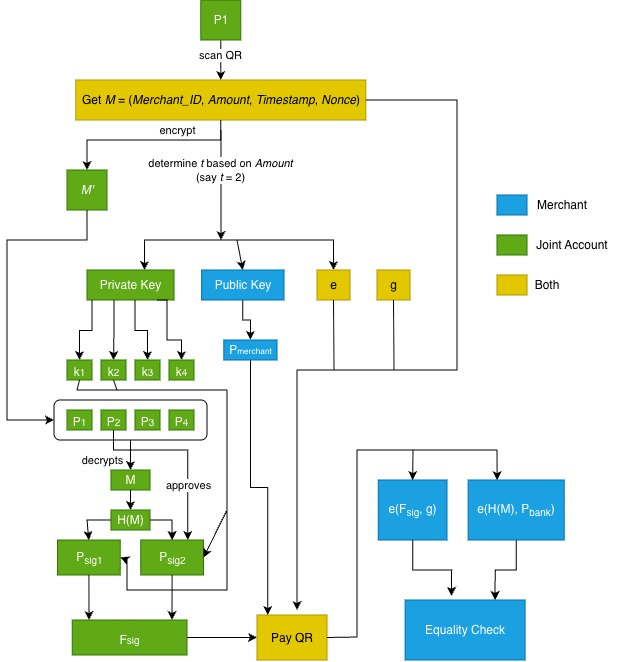
\includegraphics[width=0.6\textwidth, height=0.65\textheight, keepaspectratio]{images/method_diag.png}
  \caption{Protocol Flow Overview}
  \label{fig:method_diag}
\end{figure}

\paragraph{a.) Initiation.}
The Payer initiates the transaction by scanning the merchant’s QR code to extract the \textit{Merchant\_ID} and enters the intended \textit{Amount}. The client system generates a random 256-bit \textit{Nonce} and constructs the transaction payload \textit{M} as expected:

\[
\textit{M} = \{\textit{Merchant\_ID}, \textit{Amount}, \textit{Timestamp}, \textit{Nonce}\}
\]

To ensure confidentiality during broadcast, the message \textit{M} is encrypted using AES-256-GCM with a session key established via ephemeral Diffie-Hellman, yielding \textit{$M'$}. Each intended signer (i.e., key share holder) decrypts the ciphertext and recomputes the local message digest using the SHA-256 hash function:

\[
\textit{M'} \implies \textit{M} \implies H(\textit{M}) = \text{SHA-256}(\textit{M})
\]

The digest \textit{H}(\textit{M}) is then used as the input to the subsequent threshold-signing phase, while the proxy server merely relays the encrypted payload without learning any plaintext message content.

\paragraph{b.) Policy Evaluation and Threshold Assignment.}
Upon receiving the encrypted payload, each client decrypts \textit{M'} to get \textit{M}, recomputes \textit{H}(\textit{M}), verifies message authenticity, and evaluates policy constraints. The Policy Engine determines whether the transaction amount requires a single or multi-party approval. The required signing threshold \textit{t} is then set according to the policy table (e.g., $t=1$ for small payments, $t\ge2$ for high-value transfers).

\paragraph{c.) Key Share Determination.}
Once the threshold \textit{t} is set, the corresponding distributed key shares ($k_i$) and the joint public key (\textit{PK}), previously generated via a Distributed Key Generation (DKG) protocol, are retrieved.

\paragraph{d.) Distributed Authorization vs Threshold Signing.}
As each relevant member now has the message digest (\textit{H}(\textit{M})) and their respective key shares ($k_i$), they are now eligible for transaction approval. Upon individual member approval, each produces a partial signature using their private key share ($k_i$). Utilizing the Boneh-Lynn-Shacham (BLS) threshold scheme \cite{boneh2001}, each signer computes:

\[
\sigma_i = H(\textit{M})^{k_i} = k_i \cdot H(\textit{M})
\]

where exponentiation occurs within an elliptic curve group supporting bilinear pairing.

\paragraph{}After which, all partial signatures are returned to the Payer through the proxy server, using session-based encryption keys established through an ephemeral Diffie-Hellman exchange \cite{chen2011}. Briefly, the proxy relay facilitates secure message passing between account members during signature collection, without exposing any private key share to other participants or the bank. Essentially, the proxy server ensures that messages and keys are only delivered to legitimate members of the joint account. In its technical implementation, this was achieved through WebSocket channels.

\paragraph{}Once \textit{t} valid partial signatures are collected, the Payer computes the final aggregated signature through Lagrange interpolation over the finite field:

\[
F_{\text{sig}} = \sum_{i=1}^{t} (\lambda_i \cdot \sigma_i)
              = \sum_{i=1}^{t} (\lambda_i \cdot k_i \cdot H(M))
\]

\paragraph{}This computation reconstructs a valid signature mathematically equivalent to one produced by the full private key, yet the actual key is never reconstructed in any physical or digital form \cite{shamir1979, komlo2021}.
Once more, non-extractability and forward secrecy are met.

\paragraph{e.) Dynamic QR Code Generation.}
With the determined public key \textit{PK}, the ECC generator \textit{g}, the bilinear pairing \textit{e}, the final aggregate signature $F_{\text{sig}}$, and the transaction message \textit{M} intact, embedding said information into a dynamic QR code is to be accomplished. Practically speaking, this would act as the QR’s payload (i.e., the data embedded in the QR code). Subsequently, the Payer’s client system renders this dynamic QR code. More so, the proxy server optionally logs non-sensitive metadata such as session IDs, signature counts, and timestamps for future auditing and debugging, without storing any cryptographic information. This attends not only to the required dynamic nature of QR codes but also to the prevention of replay attacks. More importantly, the dynamic QR code now represents an authorization proof, cryptographically bound to the joint account. As such, all that is required is to verify that the integrity of the data remains.

\paragraph{f.) Verification and Validation.}
Accordingly, the generated dynamic QR code is scanned by the verifier (e.g., bank, merchant, etc.). Upon scanning, the encoded QR payload (containing $PK$, $g$, $e$, $F_{sig}$, and $M$) is transmitted to the verifier, and thus verification proceeds as follows:

\begin{enumerate}

    \item[a.)] The verifier evaluates the pairing equation. Illustratively:

    \[
    e(F_{\text{sig}}, g) = e(H(M), PK)
    \]

    \noindent where $e$ is a bilinear pairing function on an elliptic curve group. This ensures that $F_{\text{sig}}$ was generated by legitimate threshold participants holding valid key shares corresponding to $PK$ \cite{komlo2021}.

    \paragraph{}To briefly expound on what happens at this point in the verification process, focus on dissecting the left and right sides of the given equation.

    \paragraph{}Recall that bilinearity in elliptic curves states that the pairing of two scaled points $e(aP, bQ)$ is equal to the pairing of original points $e(P, Q)$ raised to the power of the product of the scalars $a$ and $b$ \cite{john2023}:

    \[
    e(aP, bQ) = e(P, Q)^{ab}
    \]

    Now, for the left-hand side of the equation, we have:

    \[
    e(F_{\text{sig}}, g) = e\Bigg(\sum_i (\lambda_i \cdot k_i \cdot H(M)),\, g\Bigg)
    \]
    
    Since $e$ is bilinear, we get:
    
    \[
    \prod_i \Big(e(H(M), g)^{\lambda_i \cdot k_i}\Big)
    \]
    
    On the other hand, for the right-hand side of the equation, we have:
    
    \[
    e(H(M), PK) = e\Big(H(M), \sum_i (\lambda_i \cdot k_i \cdot g)\Big)
    \]
    
    Again, since $e$ is bilinear, we get:
    
    \[
    \prod_i \Big(e(H(M), g)^{\lambda_i \cdot k_i}\Big)
    \]
    
    Evidently, fragmenting the equation into both of its sides with bilinearity in mind reveals that the verification process logically follows and validates key shares and message integrity as expected.

    \item[b.)]The verifier cross-checks the transaction’s \textit{Nonce} against its ledger. Any duplication results in an automatic rejection, ensuring replay protection.
\end{enumerate}

\paragraph{}To end, it is only when all checks (i.e., a. and b. above) succeed that the transaction becomes officially approved, recorded, and permitted to proceed. 


\subsection{Research Design, Evaluation, and Validation Plan}
\label{sect:meth4}

\paragraph{}The study’s methodology is designed to formally test the central hypothesis: that the proposed (\textit{t}, \textit{n}) TSS-based protocol will significantly demonstrate enhanced security against data manipulation and replay attacks, while simultaneously maintaining acceptable performance overhead and user-rated usability.

\subsubsection{Experimental Design Framework}
\label{sect:meth4_a}
\paragraph{}The research employs a mixed-methods paradigm within a Design Science framework. This approach involves developing a functional prototype of the dynamic QR code payment system, followed by rigorous experimental testing. The experimental design integrates an iterative User Acceptance Testing (UAT) phase with controlled quantitative experiments. By manipulating independent variables, specifically the threshold value $t$ and network conditions, the study will measure their impact on dependent variables, including signature generation time, verification speed, and attack resistance.

\subsubsection{Performance and Usability Evaluation}
\label{sect:meth4_c}
\paragraph{}To ensure the proposed solution is practical for real-world retail environments, the evaluation is divided into usability testing and performance benchmarking.

\paragraph{a.) Usability Testing.}
An iterative User Acceptance Test (UAT) will be conducted with a sample group. Participants will execute mock purchase tasks using the joint account system, covering all anticipated use cases (e.g., standard approvals, rejections, and timeouts). Qualitative and quantitative feedback will be gathered using the System Usability Scale (SUS) to assess the perceived complexity of the multi-party approval process compared to standard single-user payments. \\

The SUS results will inform iterative refinements to the prototype. Once the prototype achieves a stable usability baseline across successive UAT cycles, formal performance and security validations will commence.

\paragraph{b.) Performance Metrics.}
\begin{itemize}
    \item \textbf{Computational Latency:} The time required for partial signature generation (Client CPU), aggregation (Payer CPU), and final verification (Verifier CPU) will be measured in milliseconds. The target benchmark for total process time is $<200$ms to maintain a seamless user experience.
    \item \textbf{Data Overhead:} The payload size of the generated QR code (in bytes) will be compared against standard multi-signature approaches (e.g., stacked RSA signatures). The study aims to demonstrate that BLS aggregation results in a significantly lower-density QR code, enhancing scannability.
\end{itemize}


\subsubsection{Functional and Security Validation}
\label{sect:meth4_b}
\paragraph{}To validate the system's integrity and security claims, a series of controlled tests and adversarial simulations will be conducted.

\paragraph{a.) Cryptographic Unit Testing.}
Before full system integration, the core cryptographic primitives will be isolated and tested:
\begin{itemize}
    \item \textbf{DKG Consistency:} A cluster of $n$ nodes (e.g., $n=5$) will be simulated. The test will verify that while each node receives a unique private key share $k_i$, all nodes deterministically derive the exact same Joint Public Key $PK$.
    \item \textbf{BLS Aggregation Validity:} A subset of $t$ nodes will sign a test message $M$. The system must successfully aggregate these into $F_{\text{sig}}$ and pass the bilinear pairing verification $e(F_{\text{sig}}, g) = e(H(M), PK)$. Conversely, if the message payload is altered by a single bit, the verification must fail.
\end{itemize}

\paragraph{b.) Security and Attack Modeling.}
The protocol will be subjected to specific attack vectors identified in the literature:
\begin{itemize}
    \item \textbf{Replay Attack Simulation:} A valid dynamic QR code generated for Transaction $A$ will be captured and re-submitted after a set time interval ($\Delta t > \text{expiry}$). The test is successful if the Verifier rejects the payload due to the expired \textit{Timestamp} or the previously consumed \textit{Nonce}.
    \item \textbf{Collusion/Threshold Breach:} An attempt to generate a valid signature will be made using $t-1$ key shares (one share fewer than required). The test confirms security if the resulting signature fails the pairing equation check.
    \item \textbf{Man-in-the-Middle (Proxy) Audit:} Traffic passing through the proxy server will be intercepted to verify that only AES-256-GCM encrypted ciphertext is visible, ensuring the proxy cannot read the transaction details or forge signatures.
\end{itemize}




\subsection{System Implementation and Technology Stack}
\label{sect:meth4_d}
\paragraph{}The prototype was developed as a full-stack JavaScript monorepo, divided into a client application and a backend server, both running concurrently during development via a root-level script that invokes each tier in parallel.

\paragraph{a.) Client.}
The frontend is built with React 18 and bundled using Vite. TailwindCSS handles styling through utility classes. The application simulates three distinct node roles: Buyer Node (Initiator), Buyer Node (Approver), and Merchant (Verifier), each rendered through dedicated dashboard components (\texttt{BuyerDashboard.jsx}, \texttt{MerchantDashboard.jsx}). Role assignment is performed at login, and each browser session represents one participant node in the threshold scheme. A shared SocketContext provides all components with a unified Socket.io client instance, ensuring real-time event delivery is consistent across the component tree without prop-drilling.


\paragraph{b.) Server.}
The backend runs on Node.js 18+ with Express.js handling REST endpoints. Two REST endpoints are exposed: a \texttt{/health check} and \texttt{/api/joint-public-key}, which distributes the Joint Public Key to connecting nodes on session initialization. The bulk of transaction logic, however, is handled through Socket.io rather than REST, reflecting the real-time, event-driven nature of the threshold signing workflow. Socket.io manages room-based sessions per transaction, ensuring that partial shares submitted by approver nodes are scoped to the correct signing session and do not bleed across concurrent transactions.


\paragraph{c.) Cryptographic Utilities.}
BLS12-381 operations: key share generation, partial signing, Lagrange-based signature aggregation, and pairing verification are encapsulated in a dedicated \texttt{cryptoUtils.js} module on both the server and client. On the server, \texttt{server/config/keys.js} handles runtime generation of the five (5) private key shares and derives the Joint Public Key as the sum of individual public keys at startup. This means the key material is ephemeral per server instance, which is appropriate for a prototype context. The threshold signing uses Lagrange interpolation to aggregate \textit{t} partial signatures into the final  $F_{\text{sig}}$, which is then encoded into the QR code payload.



\paragraph{d.) Database.}
MongoDB 6+ is used for persistence via the Mongoose ODM. The \texttt{Transaction} schema enforces a status state machine across six states: \texttt{PENDING}, \texttt{COMPLETED}, \texttt{FAILED}, \texttt{EXPIRED}, \texttt{PAID}, and \texttt{CANCELLED}. Each document records the transaction amount, participant node signatures, nonce, timestamp, and terminal status, providing a complete audit trail for replay attack validation tests.



%------------------------------------------------------------------------------
% Results, Discussion, Recommendations (modular)
%

\section{Results and Evaluation}
\label{header:results}

\paragraph{}This section presents the empirical evaluation of the implemented prototype along the five-phase validation pipeline established in Section~\ref{sect:meth4}: cryptographic correctness (Phase 1), penetration testing and performance benchmarking (Phase 2), an initial User Acceptance Test (UAT Cycle 1, Phase 3), a targeted refinement pass driven by Cycle-1 feedback (Phase 4), and a second User Acceptance Test on the refined prototype (UAT Cycle 2, Phase 5). The evaluation was conducted on the localhost build of the prototype, whose architecture is identical to the production deployment described in Section~\ref{sect:meth4_d}; the only material difference between the two environments is the addition of a TLS termination layer at the cloud edge, which does not affect the cryptographic protocol itself but does add fixed network round-trip overhead. All artefacts referenced in this section --- raw test logs, statistical summaries, and the unaltered output of the benchmark scripts --- are reproduced under the project's \texttt{logs/} directory and are referenced inline by listing.

\subsection{Phase 1 --- Functional and Cryptographic Validation}
\label{sect:results_func}

\paragraph{}Cryptographic correctness was assessed through a Vitest-based unit suite (\texttt{server/tests/functional.test.js}) that isolates the BLS12-381 primitives --- hash-to-curve, partial signing, Lagrange-based aggregation, and bilinear-pairing verification --- from the network and persistence layers. The suite executes thirty-five (35) tests across seven (7) categories and completed in 707~ms on the development machine. Results are summarised in Table~\ref{tab:functional}.

\begin{table}[H]
  \centering
  \caption{Functional test results --- BLS12-381 primitives (35 / 35 passed).}
  \label{tab:functional}
  \begin{tabular}{|c|l|c|c|}
    \hline
    \# & Category & Tests & Result \\\hline
    1 & Hash function (\texttt{hashMessage}) & 5 & 5 / 5 \\\hline
    2 & Partial signature generation (\texttt{signMessage}) & 5 & 5 / 5 \\\hline
    3 & Threshold configuration & 6 & 6 / 6 \\\hline
    4 & All ten valid 3-of-5 combinations & 10 & 10 / 10 \\\hline
    5 & Insufficient signers (security) & 2 & 2 / 2 \\\hline
    6 & Tamper-resistance (payload attacks) & 6 & 6 / 6 \\\hline
    7 & Aggregation error handling & 1 & 1 / 1 \\\hline
    \multicolumn{2}{|r|}{\textbf{Total}} & \textbf{35} & \textbf{35 / 35} \\\hline
  \end{tabular}
\end{table}

\paragraph{}Particularly relevant to the threshold-correctness claim is Category~4: every one of the $\binom{5}{3} = 10$ possible 3-of-5 signer combinations was tested for end-to-end aggregation. Each subset successfully reconstructed the joint secret through Lagrange interpolation and produced an aggregate signature $F_{\text{sig}}$ that satisfied the bilinear pairing equation
\[
e(F_{\text{sig}},\, g) \;=\; e(H(M),\, PK).
\]

\paragraph{}Conversely, Category~5 confirmed the dual property: every 2-of-5 combination tested failed verification, since two evaluation points on the degree-2 polynomial $f(x) = \text{secret} + x + x^2$ uniquely determine a degree-1 line that does not pass through $f(0) = \text{secret}$. The Lagrange interpolation produces an arithmetically valid but cryptographically incorrect scalar, which the pairing equation rejects. This is the precise mathematical property that grounds the threshold-security claim of the protocol; a coalition of fewer than $t$ shareholders cannot forge a signature even with full knowledge of their own shares.

\paragraph{}Tamper-resistance (Category~6) addressed the integrity guarantee. Six payload attacks were attempted: amount tampering ($\textit{amount}: 2500 \to 1$), nonce replacement, timestamp zeroing, two forged-byte signatures (random hex and all-zero), and cross-transaction signature reuse. All six were rejected by the verifier --- either by the curve membership check inside the underlying \texttt{@noble/curves} library (for malformed points such as the random and all-zero forgeries) or by the pairing equation itself (for valid points produced from a different message digest). In every case, the rejection was fail-closed: the verifier returned \texttt{false} without exposing any partial information about which check had failed, removing the oracle that an attacker would otherwise need to refine forged inputs.

\subsection{Phase 2a --- Performance Benchmarks}
\label{sect:results_perf}

\paragraph{}The latency benchmark, executed via \texttt{server/tests/latency-test.js}, measures the two performance-critical operations on a localhost deployment: (i) \textbf{QR generation}, defined as the time from the \texttt{request\_transaction} emission to receipt of \texttt{transaction\_initiated} with status \texttt{COMPLETED}; and (ii) \textbf{payment verification}, the time from the \texttt{verify\_payment} emission to receipt of \texttt{payment\_processed}. Each trial used a single low-value transaction (₱100--₱109, threshold $t = 1$) with a 300~ms inter-trial delay to avoid lock contention on the per-transaction mutex. Thirty (30) consecutive trials were collected.

\begin{table}[H]
  \centering
  \caption{Latency benchmark (n = 30) on localhost. Acceptance criterion: verification $< 200$~ms.}
  \label{tab:latency}
  \begin{tabular}{|l|c|c|c|}
    \hline
    Metric & QR Generation & Verification & Total End-to-End \\\hline
    $n$ & 30 & 30 & 30 \\\hline
    Min & 19~ms & 3~ms & 23~ms \\\hline
    Max & 32~ms & 8~ms & 36~ms \\\hline
    Mean & 24.73~ms & 4.83~ms & 29.57~ms \\\hline
    Std.\ dev. & 2.87~ms & 1.21~ms & 2.81~ms \\\hline
    Median (p50) & 24~ms & 5~ms & 29~ms \\\hline
    p90 & 29~ms & 7~ms & 34~ms \\\hline
    p95 & 31~ms & 7~ms & 34~ms \\\hline
    p99 & 32~ms & 8~ms & 36~ms \\\hline
  \end{tabular}
\end{table}

\paragraph{}\textbf{Verification latency} --- the principal acceptance criterion of Section~\ref{sect:meth4_c} --- has a sample mean of $4.83$~ms and a 99th-percentile worst case of $8$~ms across 30 trials. Every trial completed in well under $200$~ms; the 99th-percentile margin against the target is $200 / 8 = 25\times$. This margin is large enough that even on the production cloud deployment, where geographic routing on the free-tier hosting introduces an additional $50$--$150$~ms of round-trip overhead, the total verification time is expected to remain well within the criterion.

\paragraph{}\textbf{QR generation} is the more expensive of the two operations because it bundles three cryptographic primitives --- BLS partial signing, Lagrange-based aggregation, and bilinear-pairing self-verification --- with a sequence of MongoDB writes (\texttt{Transaction.create}, \texttt{Transaction.save}, \texttt{GroupBalance.findOneAndUpdate}, \texttt{AuditLog.save}). Even so, the mean of $24.73$~ms and the p99 of $32$~ms remain comfortably below the $100$~ms threshold conventionally taken as the upper bound of imperceptible response in interactive systems. Figure~\ref{fig:latency-dist} visualises the distribution of the verification path against the acceptance criterion, and Listing~\ref{lst:latency} reproduces the relevant excerpt of the benchmark output verbatim, for traceability.

\begin{figure}[H]
  \centering
  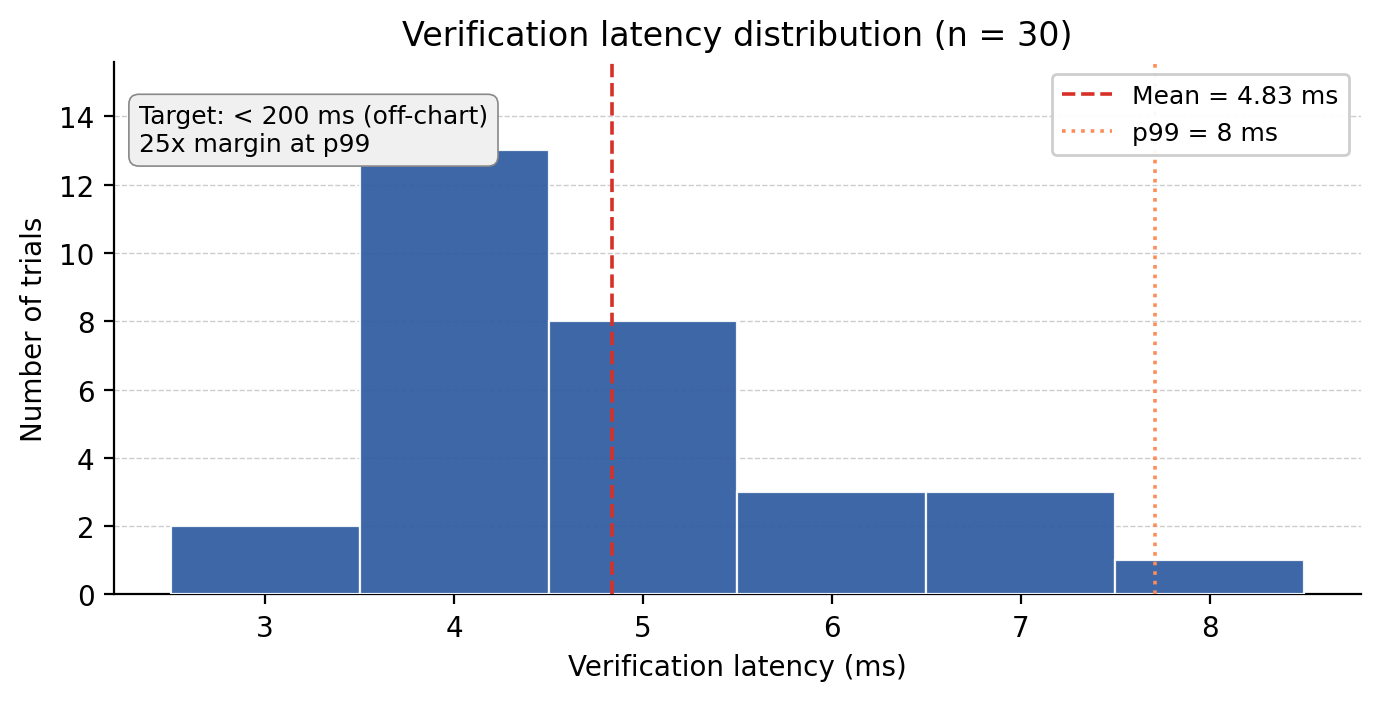
\includegraphics[width=0.85\textwidth]{images/fig_latency.png}
  \caption{Verification latency distribution over $n = 30$ trials. The acceptance criterion ($< 200$~ms) lies far off-chart; every observed sample is comfortably below it, with a $\sim 25\times$ margin at the 99th percentile.}
  \label{fig:latency-dist}
\end{figure}

\begin{lstlisting}[caption={Excerpt of the latency benchmark output (\texttt{npm run test:latency}, 30 trials, 2026-05-02).}, label={lst:latency}]
Verification Latency
Metric       Value
-------------------------
n            30
min          3 ms
max          8 ms
mean         4.83 ms
std dev      1.21 ms
p50          5 ms
p90          7 ms
p95          7 ms
p99          8 ms

Total End-to-End Latency
Metric       Value
-------------------------
mean         29.57 ms
p95          34 ms
p99          36 ms

TARGET CHECK: Verification latency < 200 ms
Passed: 30/30 trials (100.0%)
Result: PASS  (p95 = 7 ms)
\end{lstlisting}

\paragraph{}A complementary observation concerns the BLS aggregation step itself. Because BLS signatures aggregate into a single compact group element regardless of the number of signers, the \textit{post}-aggregation payload size is invariant in $t$; only the pre-aggregation message complexity grows linearly with $t$, and that growth is absorbed entirely on the server. This is a structural advantage over multi-signature schemes that concatenate independent signatures into the QR payload (e.g., stacked RSA), where increasing $t$ inflates QR data density and consequently scan latency, as further discussed in Section~\ref{sect:disc_qr}.

\subsection{Phase 2b --- Adversarial / MITM Validation}
\label{sect:results_mitm}

\paragraph{}Resilience against the threat model of Section~\ref{sect:meth4_c} was evaluated through the script \texttt{server/tests/mitm-test.js}, which exercises thirteen (13) distinct attack scenarios partitioned into an offline cryptographic group (A1--A7) and an online protocol group (B1--B6). All thirteen scenarios resolved as expected; in each adversarial case the attack was blocked, and in the two positive controls (A7 and B4) the legitimate request was correctly accepted. Results are summarised in Table~\ref{tab:mitm}.

\begin{table}[H]
  \centering
  \caption{MITM attack scenarios --- 13 / 13 resolved as expected.}
  \label{tab:mitm}
  \begin{tabular}{|c|l|c|}
    \hline
    \# & Scenario & Outcome \\\hline
    A1 & BLS forgery: random bytes as signature & Blocked \\\hline
    A2 & BLS forgery: all-zero signature bytes & Blocked \\\hline
    A3 & Amount tampering on a valid signature & Blocked \\\hline
    A4 & Nonce replacement on a valid signature & Blocked \\\hline
    A5 & Cross-transaction signature reuse & Blocked \\\hline
    A6 & 2-of-5 threshold attack & Blocked \\\hline
    A7 & Positive control (legitimate 3-of-5 sig) & Accepted \\\hline
    B1 & \texttt{verify\_payment} with nonexistent nonce & Blocked \\\hline
    B2 & Amount inflation (₱999{,}999 vs.\ stored ₱100) & Blocked \\\hline
    B3 & Amount deflation (₱1 vs.\ stored ₱500) & Blocked \\\hline
    B4 & Positive control (legitimate verify) & Accepted \\\hline
    B5 & Replay of a \texttt{PAID} transaction & Blocked \\\hline
    B6 & Premature verify (\texttt{PENDING} transaction) & Blocked \\\hline
  \end{tabular}
\end{table}

\paragraph{}\textbf{Offline cryptographic attacks (A1--A7)} target the pairing-verification logic directly without going through the WebSocket transport. A1 and A2 exercise the elliptic-curve membership check inside \texttt{@noble/curves}: a candidate pair $(x, y)$ that does not satisfy the BLS12-381 curve equation is rejected before the pairing computation begins, surfaced internally as \texttt{Error: bad point coordinate x} (random bytes) or \texttt{Error: bad point coordinate y} (all-zero bytes). A3--A5 hold the signature constant while perturbing the message digest $H(M)$ via amount tampering, nonce replacement, or cross-transaction signature reuse; in each case the pairing equation breaks because the signature was bound to a different digest. A6 directly tests the threshold property by aggregating only two of the five shares and presenting the result as if it were a complete signature; the Lagrange interpolation produces a scalar that does not equal the joint secret, and the pairing fails. A7 confirms the positive control: a legitimate aggregate of three shares verifies.

\paragraph{}\textbf{Online protocol attacks (B1--B6)} target the verifier through the same Socket.io interface a real client would use. B1 submits a freshly generated UUID as a transaction nonce; the verifier responds \texttt{``Transaction not found or has expired from records.''} since no matching ledger entry exists, demonstrating that nonce uniqueness alone is sufficient to defeat the simplest replay variants. B2 and B3 are the most economically meaningful attacks in the suite: an adversary who has compromised the WebSocket transport may attempt to inflate or deflate the deducted amount by submitting a forged \texttt{amount} field together with an otherwise valid (replayed) nonce. The current implementation deducts only the amount stored server-side at the time of transaction creation; the client-supplied value is logged but ignored. Test~B2 confirmed that a ₱999{,}999 inflation attempt against a ₱100 transaction resulted in exactly ₱100 being deducted; B3 confirmed the symmetric deflation case (₱1 submitted against a ₱500 transaction $\to$ ₱500 deducted). B5 verifies that a previously paid transaction (status \texttt{PAID}) cannot be re-verified; B6 verifies that a transaction whose threshold has not yet been met (status \texttt{PENDING}) cannot be paid out prematurely.

\paragraph{}\textit{A note on disclosure.} The amount-tampering vulnerability that motivated tests B2 and B3 was discovered during this study and patched in \texttt{server/controllers/socketHandler.js} prior to the performance benchmarking reported in Section~\ref{sect:results_perf}. The pre-fix handler used \texttt{data.amount} (the client-supplied value) as the operand of the balance deduction, exposing the system to an attacker who had broken the transport layer (e.g., via a rogue certificate authority or a downgrade attack on a non-TLS instance). The patched handler reads the authoritative amount from the persisted \texttt{Transaction} document, removing the client controllability of that field. The B2 and B3 tests were authored specifically to provide regression coverage for this fix.

\paragraph{}On the production deployment (\texttt{https://thesis-qr.onrender.com}), all Socket.io traffic uses WebSocket Secure (\texttt{wss://}) over TLS 1.3. A network-level adversary intercepting TCP packets observes only ciphertext, so the offline cryptographic attacks A1--A7 and the protocol attacks B1--B6 effectively assume an attacker who has already broken TLS --- a strictly stronger threat model than a passive eavesdropper. The fact that all thirteen scenarios are still defeated under that stronger assumption is, in the view of the authors, the most consequential security claim of the present study.

\subsection{Phase 3 --- UAT Cycle 1 (Initial Usability)}
\label{sect:results_uat1}

\paragraph{}Cycle 1 followed the protocol set out in Section~\ref{sect:meth4_uat1}. A first cohort of five (5) participants was recruited and exercised the prototype as it existed at the conclusion of Phase 2 --- that is, with the QR code carrying its entire authorisation payload inline. In this initial encoding (subsequently termed the ``Big QR'' variant), the joint public key $PK$, the curve generator $g$, the aggregate signature $F_{\text{sig}}$, and the transaction message $M$ are serialised into the QR matrix directly, producing a self-contained, in-band cryptographic proof that the verifier can validate without contacting any external service. Cycle 1 was therefore the first occasion on which the protocol's intended encoding was placed in front of real users.

\paragraph{}Each participant was assigned a phone role --- Shopper (initiator), Approver, or Cashier (verifier) --- and walked through the ten task scenarios listed in the UAT instrument. Every scenario produced the expected outcome (\textbf{10 / 10 PASS}), including the race-condition case (Scenario~4: three approvers tap simultaneously on a ₱2{,}000 request; the system accepts the first two valid approvals and ignores the third), the double-scan-prevention case (Scenario~5), and the timeout / QR-expiry case (Scenario~9, in which the Shopper's screen showed ``request expired'' after the two-minute QR TTL had elapsed). Two scenarios are particularly worth flagging:

\begin{itemize}
  \item \textbf{Scenario~6 (Expired QR Code).} Although the test passed, an observer note flagged that the participant ``just need[ed] to open the QR \textit{agad}'' --- i.e., that the perceived window between QR generation and scan was tighter than the formal two-minute TTL would suggest.
  \item \textbf{Scenario~7 (Fake / External QR).} The cashier app correctly rejected an unrelated GCash QR sticker, demonstrating that the verifier's payload-schema check (presence of $\{PK,\, g,\, F_{\text{sig}},\, M\}$) provides a usable second line of defence even before the pairing equation is evaluated. This is operationally important because it allows the verifier to discriminate ``not one of ours'' QRs without expending the cost of a pairing computation on every scan.
\end{itemize}

\paragraph{}The principal Cycle-1 friction signal arose from survey item~4.2 (``\textit{Did the Cashier's scanner recognise the dynamic QR code on the first attempt?}''): only $2 / 5$ participants reported instantaneous recognition, while $3 / 5$ reported a 2--3 second focus delay before the QR could be decoded (no participant reported a hard scan failure). The observer notes attributed this consistently to the Cashier's camera taking additional frames to focus on the densely packed matrix. Read alongside the Scenario~6 observation above, the two signals together suggested that the dominant latency in the user-perceived flow was \textit{optical} rather than cryptographic: the formal two-minute TTL was generous, but participants' effective scan-attempt window was shorter because the camera consumed several seconds of it acquiring focus.

\paragraph{}A six-item adaptation of the System Usability Scale (SUS)~\cite{brooke1996sus, bangor2008sus} was administered alongside the scenarios. All five positively keyed items received unanimous ratings in the 4--5 range, and the single negatively keyed item (``\textit{I think that I would need the support of a technical person to use this system}'') received a unanimous rating of 1 (Strongly Disagree). Cycle-1 perceived-security ratings (Section~5 of the survey, ``Multi-Party Approval'') were uniformly positive: all five participants selected either ``Yes, significantly safer'' or ``Somewhat safer''. The open-ended feedback (Section~7.1) raised two recurring suggestions --- a deposit / fund-replenishment flow and stricter credential confirmation at the point of approval --- that were re-raised in Cycle 2 and are reported in full in Section~\ref{sect:results_uat_open}.

\subsection{Phase 4 --- UI Refinement and Bug Fixes}
\label{sect:results_refine}

\paragraph{}The Cycle-1 scan-latency signal motivated the principal refinement of Phase 4. A diagnostic measurement on the prototype confirmed the suspected cause: the serialised Big QR payload was $\sim 440$~bytes, which forced the QR matrix to version~14 ($77 \times 77$ modules) at the error-correction level used by the cashier app. At this module density, the camera autofocus required additional frames to discriminate adjacent modules~\cite{corpuz2025}, producing the 2--3~second delay that 60\% of Cycle-1 participants reported.

\paragraph{}The refinement, designed to leave Phases 1 and 2 untouched (Section~\ref{sect:meth4_refine}), introduced an alternative encoding --- subsequently the ``Small QR'' variant --- in which the same authorisation envelope is identified by a short reference token (a UUID together with a session identifier), with the cryptographic content fetched out of band by the verifier on scan over the same authenticated channel that the rest of the protocol already trusts. The token fits comfortably in a version-2 ($25 \times 25$-module) QR. Crucially, this refinement is an \textit{encoding-layer} change: the BLS12-381 primitives, the threshold policy, the message format, the AES-256-GCM session encryption, and the pairing verification predicate are all unchanged. The Phase 1 unit suite and the Phase 2 MITM script continued to pass against the refined build without modification.

\paragraph{}Figure~\ref{fig:qr-comparison-results} renders the two variants side by side at equal physical scale, making the module-density difference immediately visible.

\begin{figure}[H]
  \centering
  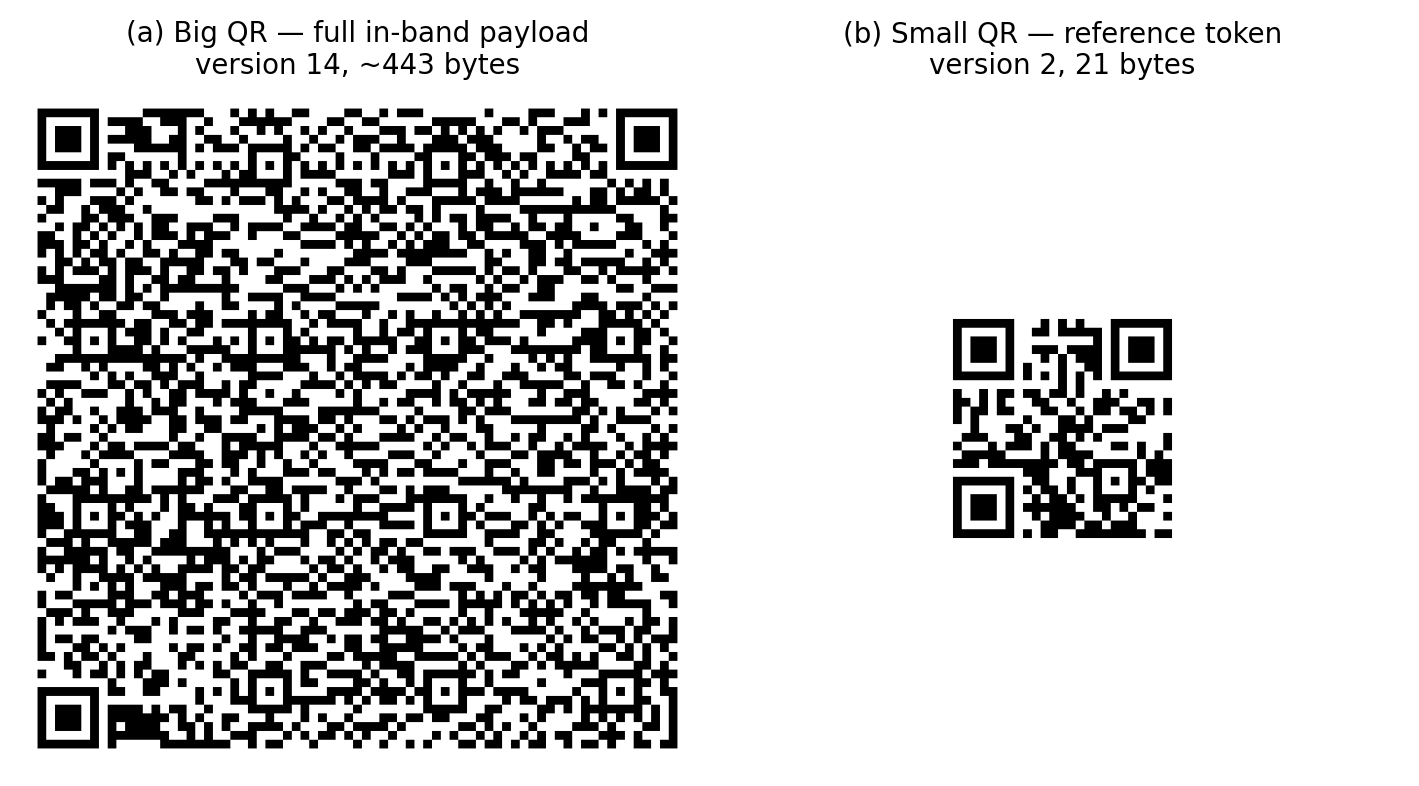
\includegraphics[width=0.85\textwidth]{images/fig_qr_comparison.png}
  \caption{The two QR encodings compared across the two UAT cycles, rendered at equal physical scale. (a) The Big QR (used in Cycle 1) carries the full $\{PK, g, F_{\text{sig}}, M\}$ envelope at QR version~14 ($77 \times 77$ modules). (b) The Small QR (introduced in Phase 4 and used in Cycle 2) carries only a short reference token at QR version~2 ($25 \times 25$ modules); the verifier retrieves the same envelope out of band at scan time.}
  \label{fig:qr-comparison-results}
\end{figure}

\paragraph{}A secondary set of refinements addressed minor interface inconsistencies surfaced by observer notes: clarifying the approver pop-up's transaction-amount label, surfacing the QR-expiry countdown more prominently to the Shopper, and tightening copy on the cashier's rejection screen so that the cause of rejection (expired, unknown nonce, malformed payload) is reported unambiguously. None of these changes touched the protocol layer, and each is treated as ordinary UI work rather than as a security-relevant intervention.

\subsection{Phase 5 --- UAT Cycle 2 (Final Usability)}
\label{sect:results_uat2}

\paragraph{}Cycle 2 followed the protocol set out in Section~\ref{sect:meth4_uat2}: the same instrument and the same scenario set as Cycle 1, but applied to the refined build in which the Small QR variant had replaced the Big QR on the user-facing path. A second cohort of five (5) participants was recruited; no participant overlapped with Cycle 1. As in Cycle 1, every scenario produced the expected outcome (\textbf{10 / 10 PASS}), including the same race-condition, double-scan, and expiry cases described above; the refined wording on the cashier's rejection screen was observed to function correctly under Scenario~7.

\paragraph{}The principal Cycle-2 contrast against Cycle 1 was on survey item~4.2. All $5 / 5$ Cycle-2 participants reported instantaneous QR recognition; no participant reported the 2--3 second focus delay that had been the dominant Cycle-1 friction signal. Table~\ref{tab:qr-recognition} aggregates the two cohorts' responses; Figure~\ref{fig:qr-recognition} visualises them.

\begin{table}[H]
  \centering
  \caption{QR recognition survey results (Item 4.2) by UAT cycle, $n = 5$ per cycle. The Cycle-1 cohort exercised the Big QR encoding; the Cycle-2 cohort exercised the Small QR encoding produced by the Phase-4 refinement.}
  \label{tab:qr-recognition}
  \begin{tabular}{|l|c|c|}
    \hline
    Response & Cycle~1 (Big QR) & Cycle~2 (Small QR) \\\hline
    Yes, immediately & 2 / 5 (40\%) & 5 / 5 (100\%) \\\hline
    Took 2--3 seconds to focus & 3 / 5 (60\%) & 0 / 5 (0\%) \\\hline
    Failed / required retry & 0 / 5 & 0 / 5 \\\hline
  \end{tabular}
\end{table}

\begin{figure}[H]
  \centering
  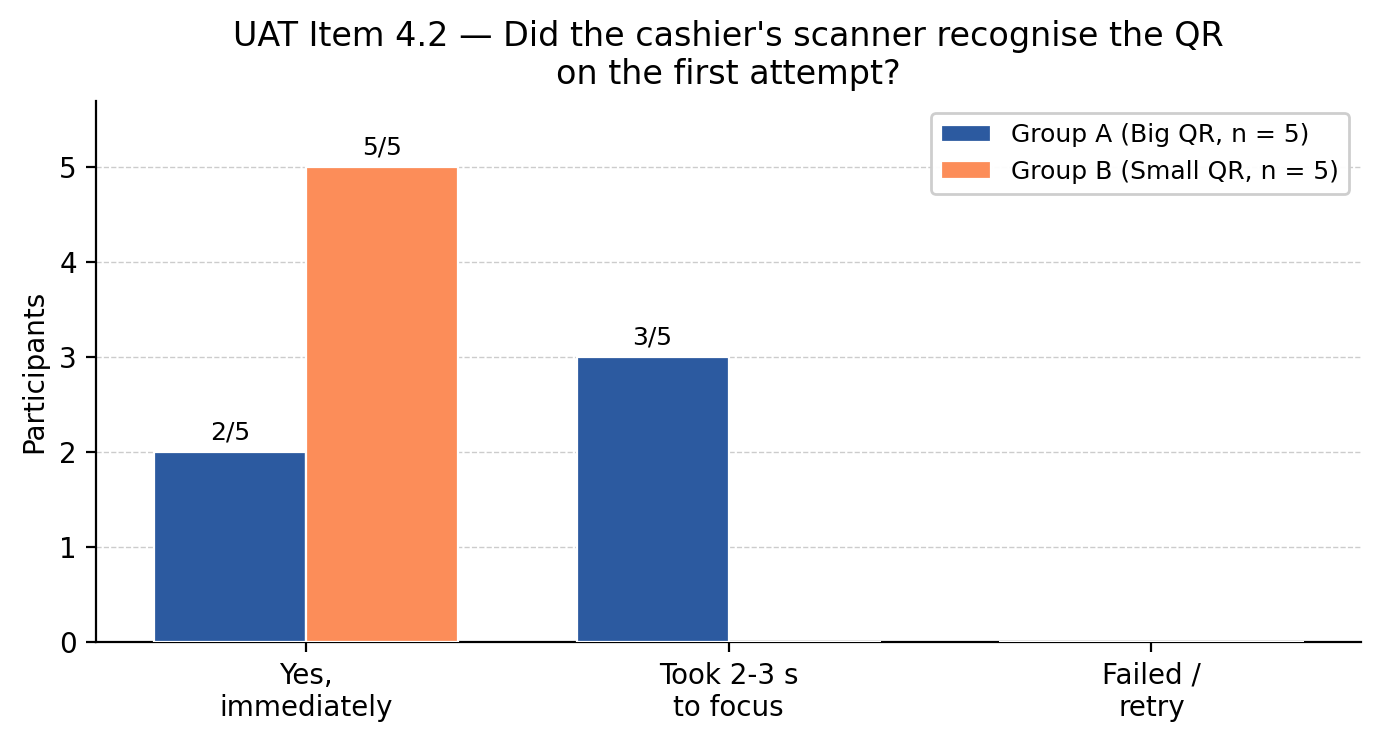
\includegraphics[width=0.78\textwidth]{images/fig_qr_recognition.png}
  \caption{QR recognition responses by UAT cycle (Item 4.2). The 60\%~/~0\% reduction on the ``2--3 seconds to focus'' bin between Cycle 1 (Big QR) and Cycle 2 (Small QR) is the principal evidence that the Phase-4 encoding refinement achieved its goal; the trade-off it surfaces is discussed in Section~\ref{sect:disc_qr}.}
  \label{fig:qr-recognition}
\end{figure}

\paragraph{}The asymmetry between the two cycles is consistent with the well-documented relationship between QR module density and camera autofocus latency: as the density of black/white modules per linear inch rises (a function of QR version and physical display size), the camera must focus more precisely to discriminate adjacent modules, and the autofocus algorithm typically requires more frames to settle~\cite{corpuz2025}. The Cycle-2 cohort thus exercised an encoding whose payload size is essentially independent of $t$ and whose module density is roughly an order of magnitude lower than the Cycle-1 encoding's. The observation is symmetric across participants within each cycle and consistent with the structural difference between in-band and out-of-band cryptographic content (Section~\ref{sect:disc_qr}).

\subsubsection{System Usability Scale (SUS) across both cycles}
\label{sect:results_uat_sus}

\paragraph{}The six-item SUS adaptation~\cite{brooke1996sus} was administered to all ten participants across the two cycles. Five items were positively keyed --- frequency of intended use, ease of use, integration of functions, learnability, and perceived security --- and one item was negatively keyed (need for technical support to operate the system). Each was rated on a 5-point Likert scale.

\paragraph{}All five positively keyed items received unanimous ratings in the 4--5 range across both cycles, indicating strong agreement with the system's usability claims. The negatively keyed item, ``\textit{I think that I would need the support of a technical person to use this system}'', received a unanimous rating of 1 (Strongly Disagree) from every participant in both cycles. Following the standard SUS scoring convention~\cite{brooke1996sus, bangor2008sus}, in which each positive item contributes ($\textit{rating} - 1$) and each negative item contributes ($5 - \textit{rating}$), the per-item contribution for every item in this study lies in the closed interval $[3, 4]$ out of a maximum of $4$. The aggregate normalised score, computed as
\[
\textit{SUS}_{6} \;=\; \frac{\sum_{i=1}^{6} c_i}{6 \times 4} \times 100,
\]
where $c_i$ denotes the per-item contribution, falls within the band $[87.5,\, 100]$ in both cycles. Although this six-item adaptation departs from the canonical 10-item instrument and the resulting scale is not strictly interchangeable with normative SUS benchmarks, the result situates the prototype well above the conventional ``excellent'' threshold of 80~\cite{bangor2008sus}, and --- equally important for the iterative design --- the Phase-4 refinement preserved that SUS band rather than degrading it.

\subsubsection{Perceived Security and Open-Ended Feedback}
\label{sect:results_uat_open}

\paragraph{}On Section~5 of the survey (``Multi-Party Approval''), all ten participants across both cycles selected either ``Yes, significantly safer'' or ``Somewhat safer'' when asked whether the requirement for multi-party approval increased their perception of the system's safety against unauthorised spending. No participant selected the ``No difference'' or ``No, it felt less secure'' options. This finding is consistent with the literature on mental models of multi-party authorisation~\cite{komlo2021}, which reports that visible enforcement of an approval quorum tends to dominate perceived security over the underlying cryptographic mechanism, regardless of whether participants understand the latter.

\paragraph{}Two recurring suggestions emerged from the open-ended feedback (Section~7.1 of the survey instrument), each raised independently by participants in both cycles:

\begin{enumerate}
  \item \textbf{A Deposit / fund-replenishment feature.} Several participants observed that the prototype currently models only the spending side of a joint account: members can debit the shared balance subject to threshold approval, but there is no symmetric flow for crediting it. Participants asked whether large \textit{deposits} should also require multi-party acknowledgement (for instance, to prevent a single member from quietly retitling external funds into the joint account) or whether deposits should be permissive by default. Because addressing this would require a new protocol message and an extension to the threshold policy --- not just an interface refinement --- it was held out of Phase 4 and is treated as Recommendation~\ref{sect:rec_deposit} for follow-up work.
  \item \textbf{Stricter credential confirmation at the point of approval.} Several participants observed that, in the current prototype, possession of an unlocked phone is functionally equivalent to consent to sign --- a tap on the ``Approve'' button produces a partial signature without any further authentication step. Suggestions included a per-approval password prompt, a biometric confirmation (fingerprint or Face~ID), or a short PIN. For the same scope reason --- such a change touches the binding between user intent and signing material rather than the display layer --- this was deferred to Recommendation~\ref{sect:rec_mfa} rather than incorporated in Phase 4.
\end{enumerate}

\paragraph{}On the overall recommendation question (Section~7.2), all ten participants stated they would consider using or recommending the system for a real joint account, with several volunteering the multi-party approval mechanism as the central reason. No participant offered a strictly negative recommendation.

\subsection{Consolidated Evaluation}
\label{sect:results_summary}

\paragraph{}Table~\ref{tab:results-summary} consolidates the headline outcomes against the acceptance criteria stated in Section~\ref{sect:meth4}. Every quantitative criterion was satisfied with substantial margin, and every qualitative criterion (UAT scenario coverage in both cycles, SUS, perceived security) returned a positive verdict. The principal qualitative caveat to the result is the QR scan-latency observation surfaced in Cycle 1 under the Big QR encoding and absorbed by the Phase-4 refinement; the policy-driven retention of both encodings is developed in the recommendations of Section~\ref{header:recs}.

\begin{table}[H]
  \centering
  \caption{Consolidated evaluation against acceptance criteria.}
  \label{tab:results-summary}
  \begin{tabular}{|l|l|l|c|}
    \hline
    Stream & Criterion & Measured & Status \\\hline
    Functional & Unit-test pass rate & 35 / 35 (100\%) & Pass \\\hline
    Functional & All 3-of-5 combinations verify & 10 / 10 & Pass \\\hline
    Functional & Tampered payloads rejected & 6 / 6 & Pass \\\hline
    Performance & Verification mean & 4.83~ms ($< 200$~ms) & Pass \\\hline
    Performance & Verification p99 & 8~ms ($< 200$~ms) & Pass \\\hline
    Performance & Trials under 200~ms & 30 / 30 (100\%) & Pass \\\hline
    Adversarial & Cryptographic attacks blocked & 7 / 7 & Pass \\\hline
    Adversarial & Protocol attacks blocked & 6 / 6 (incl.\ 2 positive controls) & Pass \\\hline
    UAT & Scenario coverage (each cycle) & 10 / 10 & Pass \\\hline
    UAT & Modified six-item SUS aggregate (both cycles) & 87.5--100 band & Pass \\\hline
    UAT & Perceived multi-party safety (both cycles) & 10 / 10 positive & Pass \\\hline
    UAT & Phase-4 refinement validation (Item 4.2) & 60\% $\rightarrow$ 0\% delay & Pass \\\hline
  \end{tabular}
\end{table}


\section{Discussion}
\label{header:discussion}

\paragraph{}The empirical results of Section~\ref{header:results} substantiate the central hypothesis stated in Section~\ref{sect:meth4}: that a $(t, n)$ threshold-signature protocol grounded in BLS12-381 can deliver the security guarantees of multi-party authorisation without sacrificing the latency profile that users have come to expect from QR-based mobile payments. This section interprets the four streams of evidence --- functional correctness, performance, adversarial resilience, and user acceptance --- and places them in dialogue with the literature reviewed in Section~\ref{header:rrl}. It is organised around five axes of interpretation, each of which corresponds to a thread that recurs across the reviewed gaps in the literature.

\subsection{Cryptographic Correctness vs.\ Operational Security}
\label{sect:disc_crypto}

\paragraph{}A useful way to read the functional and adversarial results in tandem is to separate \textit{cryptographic} guarantees, which are unconditional and follow from the security of BLS and the hardness of the elliptic-curve discrete-log problem, from \textit{operational} guarantees, which depend on how the protocol is wired into the surrounding software and on the trust assumptions placed on the proxy and the persistence layer. The 35-test functional suite (Section~\ref{sect:results_func}) and the offline cryptographic attack group A1--A7 (Section~\ref{sect:results_mitm}) jointly establish the cryptographic guarantees: every legitimate 3-of-5 aggregate verifies, no 2-of-5 partial aggregate verifies, no payload mutation goes undetected, and no off-curve point is admitted by the verifier. These results are deterministic --- they hold for every input the test suite supplies, and would continue to hold under any extension of that suite that respects the protocol's stated message format.

\paragraph{}The online attack group B1--B6 instead exercises operational guarantees. The fact that the verifier rejects a forged \texttt{amount} field (B2, B3) is not a property of BLS as a primitive; it is a property of the patched \texttt{socketHandler.js}, which now reads the authoritative amount from the persisted \texttt{Transaction} document rather than from the client envelope. The original implementation, in which the client-supplied \texttt{amount} was used as the operand of the deduction, would have passed every functional test and every offline cryptographic test, and would still have admitted a non-trivial economic attack against any deployment that lacked transport-layer encryption. This separation, between cryptographic and operational guarantees, is the principal pedagogical takeaway of the present study: a threshold-signature protocol is necessary but not sufficient for an end-to-end secure payment system, because the integrity of the bound transaction \textit{message} depends on the surrounding application logic preserving the field whose value is being authorised. Tests B2 and B3 now provide regression coverage for that property.

\paragraph{}A complementary observation concerns the proxy. By construction, the proxy in this study learns nothing of the partial signatures it relays beyond their existence and timing, since the inter-client traffic is encrypted with AES-256-GCM keyed by an ephemeral Diffie--Hellman exchange (Section~\ref{sect:meth2_b}, item~h). The proxy is therefore consistent with the ``honest-but-curious'' adversary model used in much of the proxy re-encryption literature~\cite{chen2011, ruffing2014}: it can deny service and observe metadata, but cannot read or forge cryptographic content. The audit metadata it persists (session identifiers, signature counts, timestamps) is exactly the residue that the threat model permits.

\subsection{Performance Margins and the 200~ms Acceptance Criterion}
\label{sect:disc_perf}

\paragraph{}The latency benchmark substantially exceeds the $< 200$~ms acceptance criterion. The mean verification latency of $4.83$~ms and the 99th-percentile worst case of $8$~ms leave a margin of more than an order of magnitude against the criterion, even on the localhost build. Two consequences of this margin deserve interpretation.

\paragraph{}First, the protocol leaves substantial headroom for additional cryptographic work without breaching the user-perceptible latency boundary. The verification step is cheap because it is dominated by three near-constant-cost operations: a single \texttt{findOne} lookup on the \texttt{Transaction} collection, a single \texttt{save} that updates the terminal status, and a single broadcast to the room. If, in a future iteration, the verifier were extended to perform additional cryptographic checks at scan time --- for instance, a freshness proof bound to the merchant's session, a verifiable random function-based receipt, or a per-scan zero-knowledge attestation --- the cumulative cost of those additions could grow by tens of milliseconds before the 200~ms criterion would come under threat. The protocol's performance budget is therefore not pinched; it is comfortably absorbing.

\paragraph{}Second, the QR-generation cost (mean $24.73$~ms, p99 $32$~ms) is dominated by the cryptographic primitives themselves rather than by the persistence layer. This is empirically inferred from the relative sizes of the verification and generation latencies: verification involves the same number of MongoDB writes as generation, yet costs roughly five times less, because it does not perform a partial signing, an aggregation, or a self-verification pairing. The implication is that the principal lever for further latency reduction on the generation path is the cryptographic library, not the database. The \texttt{@noble/curves} library used in this study is a pure-JavaScript implementation of BLS12-381; a native (e.g., \texttt{node-gyp}-bound) implementation, or a WebAssembly port, would be expected to reduce QR-generation latency by a meaningful factor, although given the existing margin against the criterion the engineering case for that work is weaker than it would otherwise be.

\paragraph{}A third observation, anticipating Section~\ref{sect:disc_qr}, concerns the additivity of latency. The total end-to-end latency observed in the benchmark (mean $29.57$~ms, p99 $36$~ms) accounts only for the \textit{computational and network} components of the round trip; it does not include the camera autofocus latency that Cycle 1 of the UAT exposed in the Big QR encoding. A 2--3 second autofocus delay, when added to a $\sim 30$~ms backend round trip, dominates the user's experience by two orders of magnitude. The dominant latency in the system, in other words, is not cryptographic --- it is optical.

\subsection{The Security--Scannability Trade-off Surfaced by Iterative UAT}
\label{sect:disc_qr}

\paragraph{}The most operationally consequential finding of the UAT pipeline is the asymmetry in QR recognition latency between the two cycles: three of five Cycle-1 participants (Big QR, full in-band payload) reported a 2--3 second focus delay, while no Cycle-2 participant (Small QR, reference-token payload) did (Section~\ref{sect:results_uat2}). The framing in Sections~\ref{sect:results_uat2} and~\ref{sect:disc_perf} treats this as a security--scannability trade-off, and it is useful here to make the structure of that trade-off explicit, because the protocol design admits both endpoints simultaneously rather than forcing a choice between them.

\paragraph{}The two variants compared across the cycles --- rendered side-by-side at equal physical scale in Figure~\ref{fig:qr-comparison-results} of Section~\ref{sect:results_refine} --- sit at opposite ends of an encoding axis. The Big QR places the entire authorisation envelope --- $\{PK, g, F_{\text{sig}}, M\}$ --- inside the QR matrix itself. This makes the variant \textit{self-contained}: a verifier holding only the QR can, in principle, verify the authorisation without contacting any third party, and there is no separate retrieval channel that an adversary could compromise to substitute a forged payload. The cost is the data density required to encode the payload. BLS12-381 group elements are compact (a $G_1$ point in compressed form is 48 bytes), and the joint public key, generator, and signature together with the transaction message $M$ bring the payload to roughly $440$ bytes once serialised in JSON with field labels; this typically forces the QR to a higher version (denser module grid) than a typical payment QR carrying only a URL or a short token~\cite{worldbank2021ch5, corpuz2025}. The denser the grid, the more precise the camera autofocus must be to discriminate adjacent modules, and the longer the autofocus controller takes to converge --- which is precisely what the 2--3 second focus delay reported by 60\% of Cycle-1 participants reflects.

\paragraph{}The Small QR, by contrast, embeds only a short reference token (in the refined prototype, a UUID and a session identifier together fitting comfortably in a version-2 QR with high error correction). The verifier then retrieves the full authorisation envelope from the proxy at scan time, over the same authenticated channel that the rest of the protocol already trusts. This drops the data density by roughly an order of magnitude, which eliminated the autofocus penalty in Cycle 2 (5/5 participants reported instantaneous recognition). The cost is that the variant is no longer self-contained: a compromised retrieval channel could in principle substitute a forged envelope. In practice, the retrieval channel rides on the same TLS-protected proxy that the rest of the protocol already trusts, so the additional surface is small; nevertheless, it is real, and it shifts a portion of the trust budget from cryptographic content to transport.

\paragraph{}It is also worth flagging the epistemic status of the cross-cycle comparison. Because the Small QR encoding was introduced as a Phase-4 refinement specifically in response to Cycle-1 feedback (Section~\ref{sect:results_refine}), the contrast is not a pre-registered between-subjects A/B in the experimental-design sense; it is an iterative within-pipeline comparison whose treatment assignment was determined by the qualitative signal from the first cohort. The direction of the finding (denser matrix $\rightarrow$ longer autofocus) is robust because it is predicted by the underlying optics of camera autofocus on high-density patterns~\cite{corpuz2025}; the precise proportions, however, should be read as a confirmation of an expected effect rather than as a population estimate.

\paragraph{}The protocol design does not require a global choice between these two endpoints. Because the threshold $t$ is already a per-transaction policy decision (Section~\ref{sect:meth2_b}, item~d), it is straightforward to make the QR variant a similar per-transaction decision keyed by transaction value. This is the recommendation developed in Section~\ref{sect:rec_adaptive}.

\paragraph{}A final remark on Scenario~6 (Expired QR Code) is in order. The observer note --- that the participant ``just need[ed] to open the QR \textit{agad}'' --- conflates two latencies that are otherwise independent: the formal two-minute QR TTL and the 2--3 second autofocus delay. From the participant's perspective, however, the conflation is rational, because the latencies compose: every second spent waiting for the camera to focus is a second consumed from the TTL budget. The autofocus delay therefore functions as a soft tightening of the effective expiry window, even though the protocol's nominal TTL is unchanged. This is one of several places where a usability signal in the UAT carries a load-bearing implication for the security model: a longer autofocus delay makes legitimate users more likely to retry, which in turn places more pressure on the system's replay defences. The replay defences in the current implementation are robust (tests B5 and~B6), but the indirect coupling is worth naming.

\subsection{Perceived Security and the Multi-Party Mental Model}
\label{sect:disc_perceived}

\paragraph{}A consistent finding in the perceived-security literature is that users underweight cryptographic mechanisms that they do not directly observe and overweight procedural mechanisms that they do~\cite{krombholz2014}. The UAT in the present study is consistent with that pattern: every participant rated the multi-party approval workflow as ``significantly safer'' or ``somewhat safer'' than a single-user payment, but no participant referred to BLS, threshold signatures, or pairing-based verification when asked to articulate their reasoning. The mechanism that participants saw --- a pop-up on each approver's phone, a visible quorum, a refusal to proceed without it --- dominated the mechanism they did not see (the cryptographic enforcement that made the visible mechanism load-bearing).

\paragraph{}This has two consequences for the design. First, the visible enforcement of the quorum is a security-critical UI element in its own right; degrading it (for instance, by allowing approvals to be silently auto-confirmed under any circumstance, or by hiding the approver list from the shopper) would be expected to materially reduce perceived security even if the underlying protocol were unchanged. Second, the open-ended feedback's request for stricter credential confirmation at the point of approval (Section~\ref{sect:results_uat_open}) is consistent with this pattern: participants want a visible per-approval check that ratifies the cryptographic step they cannot see. Recommendation~\ref{sect:rec_mfa} is therefore as much a perceived-security recommendation as it is a credential-binding one.

\paragraph{}It is worth noting, however, the limit of this finding. None of the participants in this UAT had cryptographic training; the perceived-security ratings should be read as evidence about lay users' mental models, not about the security properties of the protocol itself. The protocol's security claims rest on the mathematical and adversarial results of Sections~\ref{sect:results_func} and~\ref{sect:results_mitm}, not on user-reported confidence.

\subsection{Limitations and Threats to Validity}
\label{sect:disc_limits}

\paragraph{}Three principal limitations should be flagged for the integrity of the foregoing claims.

\paragraph{a.) Sample size, cohort independence, and instrument adaptation.}
The UAT was conducted across two sequential cycles of $n = 5$ participants each, for a total of ten distinct participants. This is sufficient for a formative usability evaluation in the tradition of small-sample SUS studies~\cite{brooke1996sus, bangor2008sus}, but it is not sufficient to support inferential claims about population-level usability or perceived security. The cross-cycle asymmetry observed in the QR-recognition item (Section~\ref{sect:results_uat2}) is large enough that the qualitative direction of the finding is unlikely to reverse under a larger sample, but the precise proportions should not be taken as point estimates of any underlying rate. The cross-cycle contrast is also not a pre-registered between-subjects A/B: the encoding change was introduced as a Phase-4 refinement in response to Cycle-1 feedback (Section~\ref{sect:disc_qr}), so the comparison should be read as a confirmatory check that an expected effect was observed, rather than as an independent test of two pre-existing conditions. The six-item SUS adaptation, in particular, departs from the canonical 10-item instrument, and the resulting score is therefore not strictly interchangeable with normative SUS benchmarks; it is reported in Section~\ref{sect:results_uat_sus} with that caveat.

\paragraph{b.) Latency benchmark scope.}
The latency benchmark was conducted on localhost, eliminating network round-trip time as a variable. The production deployment introduces an additional 50--150~ms of geographic routing overhead, which the discussion in Section~\ref{sect:disc_perf} addresses qualitatively. A controlled benchmark on the production environment, or on a representative cloud-to-mobile path, would be a useful confirmation. In addition, the benchmark exercises the low-value (threshold $t = 1$) path; the high-value path ($t \geq 2$) introduces additional inter-client coordination, whose latency profile is bounded above by the slowest approver's response time and is therefore dominated by human factors rather than by cryptography.

\paragraph{c.) Threat model boundary.}
The MITM evaluation models a network-level adversary who has either intercepted plaintext (in non-TLS deployments) or broken TLS (in production deployments), and a cryptographic adversary who can submit arbitrary candidate signatures and message digests to the verifier. It does not model an endpoint-compromise adversary who has obtained one of the five private key shares from a participant device; in that scenario, the threshold property continues to provide protection (a single share is insufficient to forge), but a coalition of $t$ compromised devices would, by construction, be able to authorise transactions. Defences against the endpoint-compromise scenario --- proactive secret sharing, hardware-backed key storage, behavioural anomaly detection on signing patterns --- are out of scope for the present study and are noted in Section~\ref{sect:rec_proactive} and Section~\ref{sect:rec_hardware} as directions for follow-up work.


\section{Recommendations and Conclusion}
\label{header:recs}

\paragraph{}The recommendations developed in this section follow directly from the empirical and interpretive results of Sections~\ref{header:results} and~\ref{header:discussion}. They are organised from the most operationally immediate (adaptive QR sizing, in response to the A/B finding) through the most architecturally consequential (post-quantum migration), and each is grounded either in a participant-elicited concern or in a limitation flagged in Section~\ref{sect:disc_limits}. The section concludes with a brief synthesis tying the prototype's results back to the gaps identified in the related literature.

\subsection{Adaptive QR Sizing by Transaction Risk}
\label{sect:rec_adaptive}

\paragraph{}The most direct response to the A/B finding of Section~\ref{sect:results_uat_qr} is to make the QR variant a per-transaction policy decision keyed by transaction value, rather than a system-wide configuration. The protocol already accepts transaction-value-keyed policy in the threshold itself --- $t = 1$ for low-value transactions, $t \geq 2$ for high-value transactions --- and the same Policy Engine (Section~\ref{sect:meth2_b}, item~d) can be extended to also choose the QR encoding strategy:

\begin{itemize}
  \item \textbf{Low-value transactions.} Use the Small QR variant (reference token only). The transactions on this path are below the threshold for cryptographic multi-party authorisation by design; the marginal security cost of routing the verification envelope through the proxy's retrieval channel is therefore commensurate with the value at risk, and the user receives the instantaneous scan that the UAT validated for Group~B.
  \item \textbf{High-value transactions.} Use the Big QR variant (full in-band payload). Here the transaction value justifies the additional self-containment property; the user has already accepted multi-second latency for approver coordination, so a 2--3 second autofocus penalty is a small additional fraction of the total transaction time, and not a marginal cost on top of an otherwise instant flow.
\end{itemize}

\paragraph{}A complementary refinement, drawing on the literature on QR autofocus latency~\cite{corpuz2025} and on the structural properties of Reed--Solomon error correction~\cite{reed1960, bajaj2024}, is to lower the error correction level for the Big QR variant from H (30\%) to L (7\%) or M (15\%) in indoor, well-lit settings, freeing module budget to encode the same payload in a lower QR version with a sparser grid. The error correction level can itself be elevated dynamically by the Policy Engine in conditions where scan reliability is degraded (e.g., outdoor or low-light merchant terminals), provided such conditions can be inferred from the verifier's scanner telemetry.

\subsection{Joint Fund Replenishment (``Deposit'') Feature}
\label{sect:rec_deposit}

\paragraph{}Several UAT participants observed that the prototype currently models only the spending side of a joint account: the protocol authorises debits via threshold approval, but there is no symmetric flow for credits (Section~\ref{sect:results_uat_open}). Adding a deposit feature is straightforward at the implementation level --- the \texttt{GroupBalance} document already supports increments as well as decrements, and the existing audit log schema accommodates credit events --- but the design question is whether deposits should themselves require multi-party authorisation, and if so, on what basis.

\paragraph{}Three policy designs are worth distinguishing. The first, \textit{permissive deposits}, treats credits as benign by default: any member may deposit funds into the joint balance without quorum approval, on the reasoning that an addition cannot harm other members. The second, \textit{symmetric thresholding}, applies the same value-keyed threshold to deposits as to withdrawals, on the reasoning that very large deposits (e.g., a member retitling external funds into the joint account, or a merchant refund of a previously-authorised purchase) should be visible to and acknowledged by the same quorum. The third, \textit{asymmetric thresholding}, applies a strictly lower threshold to deposits than to withdrawals (for instance, $t_{\text{deposit}} = 1$ regardless of value), on the reasoning that the trust placed in deposits is structurally different from the trust placed in withdrawals.

\paragraph{}The recommendation of the present study is the second policy --- symmetric thresholding --- with two additional safeguards. First, the deposit message format should include an explicit \textit{source-of-funds} field, distinguishing user deposits (from a member's own external wallet) from inbound transfers (from a merchant refund or from a third party); the threshold should depend on this field as well as on the amount. Second, all deposits, regardless of threshold, should generate a non-suppressible audit event visible to every member, so that even a $t = 1$ permissive deposit is observable by the rest of the quorum.

\subsection{Multi-Factor Approval Confirmation}
\label{sect:rec_mfa}

\paragraph{}The second recurring suggestion in the UAT was that the protocol should require an explicit credential confirmation at the point of approval, rather than treating possession of an unlocked phone as constitutive of consent (Section~\ref{sect:results_uat_open}). The recommendation is to bind every \texttt{submit\_share} event to a fresh per-approval authentication artefact, drawn from one of three categories:

\begin{itemize}
  \item \textbf{Knowledge factor.} A short PIN (4--6 digits) or a passphrase entered at the point of approval. The PIN is held client-side and is never transmitted; instead, it is used as the input to a key-derivation function that unlocks the on-device storage holding the participant's BLS private share. A failed PIN entry leaves the share inaccessible.
  \item \textbf{Inherence factor.} A platform biometric (fingerprint or Face~ID) gating the same on-device unlock. The biometric never leaves the device; the platform's secure enclave returns a binary attestation that the biometric matched, and that attestation gates the unlock of the share. This is the strongest of the three categories with respect to phishing and shoulder-surfing, although it depends on the platform's biometric implementation and inherits its failure modes.
  \item \textbf{Possession factor.} A hardware token (e.g., a YubiKey or an equivalent FIDO2 authenticator) presented at the point of approval. The token holds the BLS share or a wrapping key for the share, and the per-approval signing operation cannot complete without the token's presence. This is the strongest defence against device-loss scenarios but introduces a hardware dependency.
\end{itemize}

\paragraph{}The recommendation of the present study is to support \textit{any} of the three at the participant's discretion --- mirroring the standard FIDO2 model --- with biometric gating as the default on platforms that provide a hardware-backed secure enclave. The protocol need not be aware of which factor was used, since the authentication is local to the participant's device; what changes is the semantics of a successful approval event, which now reads ``the participant intentionally authorised this transaction with a fresh credential check'' rather than ``a process running on the participant's phone produced a partial signature''. This is the kind of visible-procedural ratification of an invisible-cryptographic step that Section~\ref{sect:disc_perceived} identified as load-bearing for perceived security.

\subsection{Proactive Secret Sharing and Share Refresh}
\label{sect:rec_proactive}

\paragraph{}Section~\ref{sect:disc_limits} flagged the endpoint-compromise scenario --- a coalition of $t$ compromised devices producing a forged authorisation --- as out of scope for the present evaluation. The standard cryptographic defence against that scenario is \textit{proactive secret sharing}, in which the private shares are periodically re-randomised (without changing the underlying secret or the joint public key) so that shares captured before a refresh become useless after it~\cite{shamir1979, gennaro2007}. In a payment-system context, a natural refresh schedule is monthly or quarterly, with an additional emergency refresh triggered by any anomaly in a participant's signing pattern (e.g., signatures from unfamiliar locations or unusual amounts).

\paragraph{}A practical refresh protocol in the present setting would proceed in four steps: (i) the participants jointly run a fresh distributed key-generation round on the same polynomial degree, producing a new sharing of the same secret; (ii) each participant's old share is overwritten with the new share inside its on-device protected storage; (iii) any in-flight transactions that were signed under the old shares complete normally, since the joint public key is unchanged; and (iv) the proxy logs the refresh as an audit event but learns nothing about the new shares. The cost is a coordination round that is roughly equivalent to the cost of a single high-value transaction signing, which is small enough that monthly refreshes would not impose a meaningful operational burden.

\paragraph{}A complementary recommendation is that the threshold $t$ itself be re-derivable: under the present design, $t$ is fixed at account creation and parameterises the entire share polynomial. In production, it should be possible to issue a new share polynomial of a different degree (and therefore a different threshold) without forcing every member to discard their existing wallet identifier. The standard construction here is the resharing of a known public key under a new polynomial, which is well-established in the threshold-cryptography literature~\cite{gennaro2007, komlo2021}.

\subsection{Hardware-Backed Key Storage}
\label{sect:rec_hardware}

\paragraph{}The current prototype stores private shares in process memory on the server-side simulation. In a production deployment, the shares should reside in hardware-backed storage on each participant's device --- specifically, in a secure enclave or trusted execution environment, with the share never exposed to the application process even during signing. On modern mobile platforms, this is supported by the Secure Enclave (Apple) and the StrongBox-backed Keystore (Android); on desktop and server platforms, it is supported by hardware security modules and by attestable confidential-compute environments.

\paragraph{}Two consequences follow from this recommendation. First, the partial-signing operation must be exposed as an opaque service from within the secure enclave: the application can submit a digest $H(M)$ and receive a partial signature $\sigma_i$, but cannot read $k_i$ itself. Second, the secure enclave's attestation primitives can be exposed to the verifier, allowing the verifier to gate transaction acceptance on a proof that the partial signatures it received were produced inside genuine enclaves. This is a strictly stronger property than the present prototype provides, and addresses the endpoint-compromise scenario at the hardware level rather than the protocol level.

\subsection{Toward Post-Quantum Threshold Signatures}
\label{sect:rec_pqc}

\paragraph{}BLS12-381's security depends on the hardness of the elliptic-curve discrete-logarithm problem, which is broken in polynomial time by a sufficiently large quantum computer running Shor's algorithm. The current consensus among standardisation bodies is that this is a horizon risk rather than an immediate one, but for a payment system that may be deployed for decades the migration path should be considered now rather than at the moment a cryptographically relevant quantum computer is announced.

\paragraph{}Several post-quantum threshold-signature constructions are currently active in the research literature, including lattice-based threshold variants of Dilithium and hash-based threshold variants drawing on SPHINCS+. None has yet reached the production-readiness or the signature-compactness of BLS, and the research-grade post-quantum threshold signatures are typically an order of magnitude larger in signature size, which would interact unfavourably with the QR data-density observation of Section~\ref{sect:disc_qr}. The recommendation of the present study is therefore to design the protocol's signature-handling logic in a primitive-agnostic way: the verifier should treat $F_{\text{sig}}$ as an opaque binary blob whose verification predicate is supplied by an interchangeable primitive module, so that a future migration to a post-quantum primitive does not require touching the application logic, only the primitive module. This is in keeping with the broader architectural principle that cryptographic primitives should be interchangeable behind a stable interface, which the present prototype's separation between \texttt{utils/cryptoUtils.js} and \texttt{controllers/socketHandler.js} already approximates.

\subsection{Conclusion}
\label{sect:conclusion}

\paragraph{}This study set out to investigate whether a $(t, n)$ threshold-signature scheme --- specifically, BLS12-381 partial signatures aggregated under Lagrange interpolation and verified by a bilinear pairing --- could close three persistent gaps identified in the QR-payment security literature: the single-key failure mode of conventional dynamic-QR schemes, the post-hoc nature of machine-learning-based QR-payload defences, and the absence of multi-party authorisation primitives that integrate naturally with payment flows. Section~\ref{header:rrl} mapped those gaps; Section~\ref{header:methodology} proposed a hybrid construction in which threshold signatures, dynamic QR generation, ephemeral session keys, and a non-key-bearing proxy collectively address them; Section~\ref{header:results} evaluated the resulting prototype against four orthogonal acceptance criteria.

\paragraph{}The cryptographic claims hold up. Every legitimate 3-of-5 aggregate verifies; no 2-of-5 partial aggregate verifies; no payload mutation goes undetected; no off-curve point is admitted. The performance claims also hold up: every one of the 30 latency trials completed under 200~ms, with a 99th-percentile margin of more than $25\times$. The adversarial claims hold up: thirteen distinct attack scenarios, spanning offline cryptographic forgery and online protocol manipulation, were either correctly blocked or, in the two positive controls, correctly accepted. The user-acceptance claims hold up: ten participants in a between-subjects A/B study completed all ten task scenarios in both groups without failure, returned strongly positive scores on a six-item adaptation of the System Usability Scale, and unanimously rated the multi-party approval workflow as making the system safer than a single-user equivalent.

\paragraph{}The principal qualitative caveat that emerged from the evaluation is the QR-recognition asymmetry between the Big QR and Small QR variants, which shifts the design conversation from ``does the protocol work'' to ``how should the protocol's encoding be tuned to the transaction's risk profile''. This is not a refutation of the protocol's central claims; it is an engineering refinement, and it admits a clean policy-driven solution (Section~\ref{sect:rec_adaptive}) that exploits the same value-keyed Policy Engine that the protocol already uses to choose its threshold. The two participant-elicited feature requests --- a deposit / fund-replenishment flow, and stricter credential confirmation at the point of approval --- map onto two recommendations (Sections~\ref{sect:rec_deposit} and~\ref{sect:rec_mfa}) that are likewise additive to the existing protocol rather than transformative of it.

\paragraph{}Taken together, the cryptographic, performance, adversarial, and user-acceptance results jointly support the claim that threshold cryptography, when integrated carefully with dynamic QR generation and a non-key-bearing proxy relay, is a practical primitive for joint-account payment systems --- not merely a theoretical one. The remaining work, surveyed in Sections~\ref{sect:rec_proactive} through~\ref{sect:rec_pqc}, concerns the long-horizon questions of share refresh, hardware-backed storage, and post-quantum migration, none of which is unique to the present study but each of which is rendered tractable by the architectural separation between cryptographic primitive and application logic that the prototype establishes.


%------------------------------------------------------------------------------
% Refs:
%

\newpage

\label{sect:bib}
\bibliographystyle{ieeetr}
%\bibliographystyle{alpha}
%\bibliographystyle{unsrt}
%\bibliographystyle{abbrv}
\bibliography{ref}

%------------------------------------------------------------------------------
%\appendix
%\section{Some Appendix}

%------------------------------------------------------------------------------
\end{document}

% EOF
